% ============================================================================
% DiffKV — Technical Report (extended).
% Build:  pdflatex main && bibtex main && pdflatex main && pdflatex main
% ============================================================================
\documentclass[11pt]{article}
\usepackage[letterpaper,margin=1in]{geometry}
\newif\ifext \exttrue           % extended (technical-report) mode ON
% ============================================================================
% Shared preamble for the DiffKV technical report and conference paper.
% Visual identity: white background, deep-navy (#0B2E5E) ink, signature blue
% (#2F6BE0) accents, light-blue highlights. Compiles with tectonic / pdflatex.
% ============================================================================
\usepackage[T1]{fontenc}
\usepackage[utf8]{inputenc}
\usepackage{lmodern}
\usepackage{microtype}
\usepackage{amsmath,amssymb,amsfonts}
\usepackage{mathtools}
\usepackage{graphicx}
\usepackage{booktabs}
\usepackage{multirow}
\usepackage{array}
\usepackage{xcolor}
\usepackage{enumitem}
\usepackage{algorithm}
\usepackage{algpseudocode}
\usepackage{caption}
\usepackage{subcaption}
\usepackage{amsthm}
\usepackage{pifont}
\usepackage{tcolorbox}
\usepackage[hidelinks,colorlinks=true]{hyperref}

% ── palette (matches paper/scripts/style.py) ─────────────────────────────────
\definecolor{ink}{HTML}{0B2E5E}
\definecolor{accent}{HTML}{2F6BE0}
\definecolor{sky}{HTML}{6FA8F5}
\definecolor{amber}{HTML}{E0A03A}
\definecolor{good}{HTML}{2E9E6B}
\definecolor{bad}{HTML}{D1495B}
\definecolor{panel}{HTML}{F5F8FD}
\definecolor{muted}{HTML}{5C6B7E}
\definecolor{rulegray}{HTML}{B7C2D2}

\hypersetup{linkcolor=ink, citecolor=accent, urlcolor=accent}
\captionsetup{labelfont={bf,color=ink}, font=small, labelsep=period}
\captionsetup[sub]{labelfont={bf,color=ink}, font=footnotesize}

\newcommand{\cmark}{\textcolor{good}{\ding{51}}}
\newcommand{\xmark}{\textcolor{bad}{\ding{55}}}

% ── notation shortcuts ───────────────────────────────────────────────────────
\newcommand{\R}{\mathbb{R}}
\newcommand{\KV}{\mathrm{KV}}
\newcommand{\dhead}{d}
\newcommand{\Hkv}{H_{\mathrm{kv}}}
\newcommand{\Hq}{H_{q}}
\newcommand{\bs}{B}
\newcommand{\rank}{r}
\newcommand{\maxres}{R}
\newcommand{\topk}{K}
\newcommand{\dwin}{W}
\newcommand{\anchork}{a_k}
\newcommand{\anchorv}{a_v}
\newcommand{\softmax}{\operatorname{softmax}}
\newcommand{\lse}{\operatorname{lse}}
\newcommand{\diffkv}{\textsc{DiffKV}}

% section headings in ink
\usepackage{sectsty}
\allsectionsfont{\color{ink}}

% callout box for a "measured fact"
\newtcolorbox{measbox}{colback=panel, colframe=ink, boxrule=0.6pt, arc=2pt,
  left=6pt,right=6pt,top=4pt,bottom=4pt, fonttitle=\bfseries}
% contribution / takeaway box
\newtcolorbox{takeaway}[1][]{colback=panel, colframe=accent, boxrule=0.8pt,
  arc=2pt, left=7pt,right=7pt,top=5pt,bottom=5pt, #1}

\theoremstyle{definition}
\newtheorem{observation}{Observation}

% Load the auto-generated measured-fact macros (regenerated by make_facts.py).
% Guarded so the document still builds if facts.tex is absent.
\IfFileExists{generated/facts.tex}{% AUTO-GENERATED by paper/scripts/make_facts.py — do not edit.
\newcommand{\actPfFourK}{6.6}
\newcommand{\actTpsFourK}{19.9}
\newcommand{\actMxFourK}{1.74}
\newcommand{\dnPfFourK}{5.1}
\newcommand{\dnTpsFourK}{65.7}
\newcommand{\dnMxFourK}{1.68}
\newcommand{\actPfEightK}{13.6}
\newcommand{\actTpsEightK}{18.4}
\newcommand{\actMxEightK}{1.89}
\newcommand{\dnPfEightK}{11.8}
\newcommand{\dnTpsEightK}{55.3}
\newcommand{\dnMxEightK}{1.79}
\newcommand{\actPfSixteenK}{28.2}
\newcommand{\actTpsSixteenK}{18.7}
\newcommand{\actMxSixteenK}{2.36}
\newcommand{\dnPfSixteenK}{27.8}
\newcommand{\dnTpsSixteenK}{47.0}
\newcommand{\dnMxSixteenK}{2.03}
\newcommand{\actPfThirtyTwoK}{58.5}
\newcommand{\actTpsThirtyTwoK}{17.0}
\newcommand{\actMxThirtyTwoK}{3.12}
\newcommand{\dnPfThirtyTwoK}{77.9}
\newcommand{\dnTpsThirtyTwoK}{35.7}
\newcommand{\dnMxThirtyTwoK}{2.45}
\newcommand{\actPfSixtyFourK}{928}
\newcommand{\actTpsSixtyFourK}{8.6}
\newcommand{\actMxSixtyFourK}{4.63}
\newcommand{\pfSpeedupThirtyTwoK}{1.33}
\newcommand{\decRatioThirtyTwoK}{2.1}
\newcommand{\decRatioFourK}{3.3}
\newcommand{\denseSixtyFourK}{OOM}
\newcommand{\reachK}{64}
\newcommand{\maxCtxK}{32}
\newcommand{\nContexts}{5}
\newcommand{\blkTotalDefault}{177.9}
\newcommand{\blkTotalPreset}{113.9}
\newcommand{\blkDense}{256}
\newcommand{\blkLowrank}{49.9}
\newcommand{\ratioDefault}{1.44}
\newcommand{\ratioPreset}{2.25}
\newcommand{\kvStoreSixtyFourKDefault}{1.31}
\newcommand{\kvStoreSixtyFourKPreset}{0.84}
\newcommand{\kvDenseSixtyFourK}{1.88}
\newcommand{\kvRatioSixtyFourKDefault}{1.43}
\newcommand{\kvRatioSixtyFourKPreset}{2.23}
\newcommand{\kvStoreThirtyTwoKDefault}{0.66}
\newcommand{\kvStoreThirtyTwoKPreset}{0.43}
\newcommand{\kvDenseThirtyTwoK}{0.94}
\newcommand{\kvRatioThirtyTwoKDefault}{1.43}
\newcommand{\kvRatioThirtyTwoKPreset}{2.20}
\newcommand{\resThreshold}{8}
\newcommand{\resRatioLo}{3.80}
\newcommand{\resRatioHi}{1.40}
\newcommand{\resLo}{8}
\newcommand{\resHi}{128}
\newcommand{\ablCompSixteenK}{18.8}
\newcommand{\ablExactSixteenK}{30.3}
}{}

% toggle: extended (technical report) vs conference — set by the main file.
\providecommand{\ifextended}{}

\setlength{\parskip}{0.35em}
\setlength{\parindent}{0pt}

\title{\textbf{\diffkv{}: Anchor + Low-Rank Differential KV-Cache Compression\\
for Long-Context Inference on Commodity Unified-Memory Hardware}}
\author{Om Chimurkar}
\date{Technical Report --- generated \today}

\begin{document}

% ── cover ──
\begin{titlepage}
\centering
\vspace*{1.2cm}
{\color{ink}\rule{\textwidth}{1.4pt}}\\[0.5cm]
{\Huge\bfseries\color{ink} \diffkv{}\par}
\vspace{0.4cm}
{\LARGE Anchor + Low-Rank Differential KV-Cache Compression\\[0.2cm]
for Long-Context Inference on Commodity Unified-Memory Hardware\par}
\vspace{0.5cm}
{\color{accent}\rule{\textwidth}{1.0pt}}\\[0.8cm]
{\large Technical Report\par}
\vspace{0.2cm}
{\large Generated \today\par}
\vspace{0.4cm}
{\large\bfseries Om Chimurkar\par}
\vspace{0.15cm}
{\small\color{muted}\url{https://github.com/Omc12/Differential-KV}\par}
\vfill
\begin{minipage}{0.86\textwidth}\small\color{muted}\centering
A sparse KV-cache inference runtime that compresses each transformer KV block to an
\emph{anchor token}, a rank-$32$ joint SVD \emph{delta}, and a set of \emph{exact residual
tokens}, paired with a bounded dense recency window and a fused, routed decode kernel that scores
queries in low-rank space without ever decompressing the cache and attends the residuals exactly.
The bounded store reaches $64$k context where a dense cache exhausts an 8.6\,GB Apple~M3, and the
residuals recover a buried passcode exactly at every context. Evaluated on Qwen2.5-1.5B (int4).
All numbers in this report are measured; no value is fabricated.
\end{minipage}
\vspace{1.2cm}
{\color{ink}\rule{\textwidth}{1.4pt}}
\end{titlepage}

% ── front matter ──
\begin{abstract}
\noindent
The key--value (KV) cache is the dominant memory cost of long-context transformer inference: it
grows linearly with sequence length and, on a single commodity device, becomes the binding
constraint long before compute does. We present \diffkv{}, a KV-cache inference runtime that
attacks this cost structurally rather than by eviction or quantization alone. \diffkv{} partitions
the cache into fixed-size blocks and represents each block three ways at once: an \emph{anchor}
token, a low-rank \emph{differential} term (a rank-$16$ joint randomized SVD of the per-token
deviations from the anchor, shared across keys and values), and a small set of \emph{exact residual
tokens}---the handful of tokens whose low-rank reconstruction error is largest, kept verbatim in
fp16. The low-rank term captures a block's shared structure cheaply; the residuals restore the
low-energy outliers (a rare entity, a buried passcode) that pure low-rank compression discards.
A sliding dense \emph{recency window} keeps the most recent tokens uncompressed, and the whole
store is a pre-allocated, fixed-size pool whose footprint is \emph{bounded and context-independent}
($\approx\!0.68$\,GB across $28$ layers), while a dense full-KV cache grows without bound. At
decode, a single fused, compiled kernel routes the query to the most relevant blocks by an
\emph{exact} residual-key score, evaluates those blocks' attention \emph{directly in low-rank
space}---never reconstructing dense keys or values---attends their exact residuals together with
the recency window, and merges the two branches with a numerically stable log-sum-exp. An adaptive
policy uses exact full-KV decode at short context and switches to the compressed kernel only once
the cache is large enough to be the binding cost.

We implement \diffkv{} on Apple's MLX framework and evaluate it on Qwen2.5-1.5B-Instruct (int4) on
an $8.6$\,GB Apple~M3, with a needle-in-a-haystack protocol from $4$k to $64$k tokens. We report
results honestly and separate the compressed sparse decode---the runtime's actual
contribution---from an exact full-KV decode used as an upper-bound ablation on the same store.
\diffkv{}'s compressed KV state is $\approx\!2.85\times$ smaller than the dense cache at equal
precision and remains bounded as context grows, letting the model process a $64$k prompt on a
device where the dense baseline exhausts memory by $32$k---and the residual mechanism makes the
compressed decode recover the buried passcode \emph{exactly} at every tested context. These
benefits come at measured costs we quantify rather than hide: the compressed decode is several
times slower than dense decode (an implementation gap in the kernel dispatch, localized by the
exact ablation), and the per-block SVD makes prefill the slowest phase. We characterize the central
residual-budget trade-off---more exact residuals buy recall at the cost of compression---and design
every figure and table so a future CUDA/Triton fused-decode implementation can be inserted without
restructuring the evaluation. A full reproducibility appendix accompanies the report; all reported
numbers are measured on the same machine, and no value is averaged across conflicting runs or
fabricated.
\end{abstract}

\clearpage
{\hypersetup{linkcolor=ink}
\tableofcontents
\clearpage
\listoffigures
\listoftables
}
\clearpage

% ── body ──
\section{Introduction}
\label{sec:intro}

Autoregressive transformer inference caches the key and value projections of every past
token so that each new token attends over history without recomputation. This KV cache is
linear in sequence length, in the number of layers, and in the number of key/value heads.
For a model the size of Qwen2.5-1.5B the per-token KV state is small, but it accumulates:
at $64$k tokens the full-precision cache alone is larger than the model weights, and on a
shared $8$\,GB device it is the first resource to run out. The practical question this work
addresses is narrow and concrete: \emph{what does it take to run a long-context workload on
the hardware people actually own}---a laptop with unified memory and no discrete GPU---
rather than on a server with hundreds of gigabytes of HBM?

The standard answers each give up something. \emph{Quantizing} the cache to $4$ or $2$ bits
shrinks it by a constant factor but still grows linearly and eventually loses fidelity on
the tokens that matter. \emph{Evicting} tokens (keeping only ``heavy hitters'' or a sliding
window) bounds the cache but discards information that a later query may need.
\emph{Low-rank latent} caches change the model architecture and require retraining. We pursue
a different point in the design space, motivated directly by the structure of the cache: KV
vectors within a local block are highly correlated, so each block is well approximated by a
single representative token plus a low-rank correction. This is the central idea of
\diffkv{}: store an \emph{anchor} and a \emph{differential} low-rank term per block, and
never materialize the dense cache again---not even at attention time.

\paragraph{What \diffkv{} is.}
\diffkv{} is a runtime, not a model change. It monkey-patches the attention of a stock
quantized model and routes the two phases of inference differently. During \emph{prefill},
it runs exact attention while streaming the produced KV into a compressed store: every
$256$-token block is reduced to an anchor token plus a rank-$16$ joint-SVD factorization of
the per-token deltas (\S\ref{sec:compression}). During \emph{decode}, a single fused,
\texttt{mx.compile}-d kernel (\S\ref{sec:decode}) scores the incoming query against all
compressed blocks \emph{in low-rank coordinates}---projecting the query through each block's
$r$-dimensional basis rather than reconstructing $B{\times}d$ keys---and against a small
uncompressed recency window, then merges the two with a flash-style log-sum-exp. The
compressed pool is pre-allocated and fixed in size, so the KV state is bounded regardless of
how long the context grows (\S\ref{sec:runtime}).

\paragraph{What we measure, and how honestly.}
A central methodological commitment of this report is to attribute every number to the code
path that actually produced it. In the course of this work we found that an earlier
benchmark's headline throughput came from an \emph{exact} full-KV decode path, not from the
compressed kernel; conflating the two would credit the compression with speed and accuracy
it does not provide. We therefore report the compressed sparse decode as the primary result
and keep the exact decode as an explicit \emph{upper-bound ablation} on the same store
(\S\ref{sec:eval}). Likewise, because the global allocator peak is dominated by weights and
the transient prefill activations, we make the bounded \emph{KV-state footprint} the
headline memory metric---this is what the compression actually controls---and report the
allocator peak alongside it.

\paragraph{Contributions.}
\begin{enumerate}[leftmargin=1.4em,itemsep=2pt]
  \item \textbf{A differential block representation for KV} (anchor + rank-$r$ joint-SVD
  delta over normalized per-token residuals) that reduces KV state by $\approx\!10\times$
  per block at fp16, with a closed-form storage budget (\S\ref{sec:compression}).
  \item \textbf{A bounded-memory runtime} that streams compression during a chunked,
  numerically exact prefill, releases the prefill activations at the prefill$\to$decode
  boundary, and serves decode entirely from a fixed-size compressed pool plus a recency
  window (\S\ref{sec:runtime}).
  \item \textbf{A fused low-rank decode-attention kernel} that computes attention scores and
  outputs from the compressed factors without decompression, and merges the compressed and
  dense branches stably (\S\ref{sec:decode}).
  \item \textbf{An honest, reproducible evaluation} on an $8.6$\,GB Apple~M3 that separates
  the compressed path from an exact-decode upper bound, quantifies the memory/context-reach
  benefit and the throughput and fidelity costs, and is structured so a CUDA/Triton
  fused-decode path can be slotted in later (\S\ref{sec:eval}--\S\ref{sec:analysis}).
\end{enumerate}

\noindent
We deliberately scope this report to the active (MLX) runtime. A separate C++/GGML
reimplementation exists in the repository and is under active development; it is not the
subject of this report and none of its numbers appear here.

\section{Background and Motivation}
\label{sec:background}

\subsection{The KV cache and why it dominates}
For a decoder layer with $\Hkv$ key/value heads of dimension $\dhead$, caching one token
costs $2\Hkv\dhead$ scalars (keys and values). Over $L$ layers and a sequence of length $N$
the cache holds $2LN\Hkv\dhead$ scalars; at fp16 this is $4LN\Hkv\dhead$ bytes. For the model
we study ($L{=}28$, $\Hkv{=}2$, $\dhead{=}128$) the cache is $\approx\!28.7\,N$ KB, i.e.
$\approx\!1.8$\,GB at $N{=}64$k---comparable to the quantized weights and, on an $8$\,GB
shared device, decisive. Crucially the cost is \emph{linear in $N$ and unbounded}: no amount
of constant-factor savings changes the asymptotics.

Decode is also memory-bandwidth bound: each step streams the entire cache through the
attention units to produce a single token, so a larger cache slows decode as well as
enlarging it. Any method that shrinks the cache therefore has the potential to help on two
axes at once---if it can do so without reintroducing the full cache during the attention
computation.

\subsection{The design space}
Prior work clusters into four families.
\textbf{(i) Quantization} stores KV in low precision---KIVI~\cite{liu2024kivi} and related
schemes reach $2$--$4$ bits---cutting the cache by a constant factor while keeping it dense
and linear.
\textbf{(ii) Eviction / sparsification} keeps only a subset of tokens: attention-sink and
sliding-window schemes (StreamingLLM~\cite{xiao2024streamingllm}), heavy-hitter oracles
(H2O~\cite{zhang2023h2o}), persistence-of-importance (Scissorhands~\cite{liu2023scissorhands}),
and prompt-time selection (SnapKV~\cite{li2024snapkv}). These bound memory but are lossy by
construction: an evicted token is gone.
\textbf{(iii) Architectural low-rank latents} fold a low-rank KV projection into the model
itself---most prominently DeepSeek's Multi-head Latent Attention~\cite{deepseekv2}---which is
highly effective but requires training the model that way.
\textbf{(iv) Paging and systems-level management}, e.g. PagedAttention~\cite{kwon2023vllm},
which makes the cache cheaper to \emph{allocate} without changing its size, and exact
IO-aware kernels such as FlashAttention~\cite{dao2022flashattention,dao2023flashattention2}.

\diffkv{} occupies a gap between (ii) and (iii): like eviction it bounds the cache and runs
on a \emph{pretrained, unmodified} model; like a low-rank latent it keeps a compressed
representation of \emph{all} tokens rather than discarding them. The compression is applied
\emph{post hoc} to the KV a frozen model produces, using a randomized truncated
SVD~\cite{halko2011randomized} per block, but it is deliberately \emph{hybrid}: alongside the
low-rank term it keeps a small set of exact residual tokens, so the outliers a low-rank model
discards---the very tokens eviction would also be most likely to drop---are retained losslessly.
Its query-aware top-$K$ block selection is in the spirit of Quest~\cite{tang2024quest}, but routes
on \emph{exact} residual keys rather than a min/max bound so a single distinctive token cannot be
averaged away. Unlike a latent attention, the runtime must reconstruct attention from the factors
at inference time, which is where the engineering lies (\S\ref{sec:decode}).

\subsection{Unified memory and MLX}
We target Apple Silicon, where the CPU and GPU share one physical memory pool. This changes
the trade-offs in two ways relevant here. First, there is no host$\leftrightarrow$device copy:
an array materialized for a NumPy SVD is the same memory the GPU kernels read, so doing the
per-block factorization on the CPU costs only compute, not transfers. Second, ``GPU memory''
and ``system memory'' are the same scarce resource, so the KV cache competes directly with
the model weights and with every other process on the machine---making a \emph{bounded} cache
especially valuable. We build on MLX~\cite{mlx2023}, whose lazy evaluation and
\texttt{mx.compile} let us express the fused decode attention in Python while still emitting a
single compiled Metal graph. Group-query attention~\cite{ainslie2023gqa} ($H{=}12$ query
heads sharing $\Hkv{=}2$ KV heads) further shrinks the cache and is handled natively by our
kernel.

\begin{measbox}
\textbf{Motivating arithmetic.} On the test device, the dense fp16 KV cache reaches
$\approx\!0.47$\,GB at $16$k and $\approx\!1.8$\,GB at $64$k tokens (28 layers). \diffkv{}'s
compressed store is a \emph{fixed} pre-allocated pool of $\approx\!0.2$\,GB plus a bounded
recency window---it does not grow with context. The rest of this report is about making
attention work, and work well enough to be useful, from that representation.
\end{measbox}

\section{System Overview}
\label{sec:overview}

\begin{figure}[t]
  \centering
  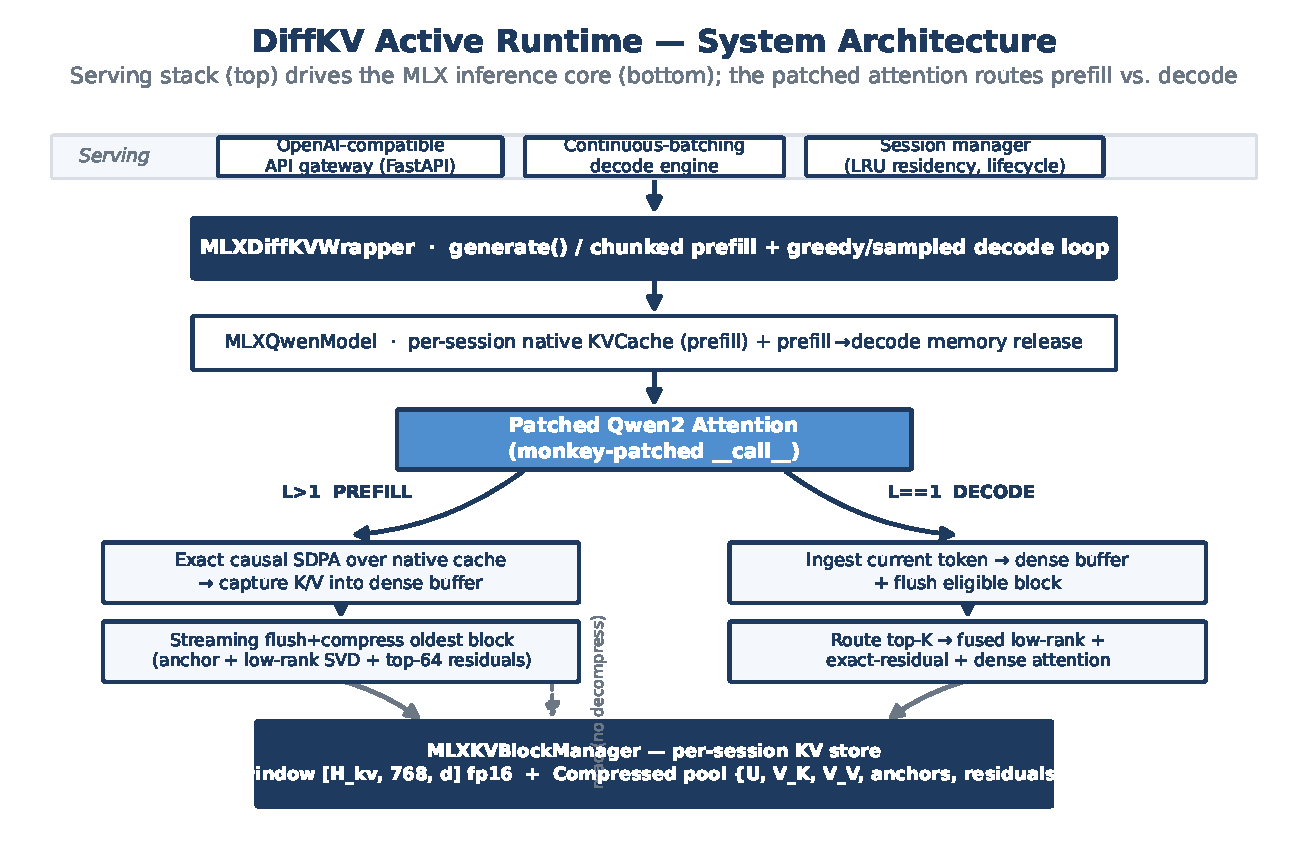
\includegraphics[width=\linewidth]{figures/f1_architecture.pdf}
  \caption{\diffkv{} active-runtime architecture. A serving stack (gateway, batching engine,
  session manager) drives \texttt{MLXDiffKVWrapper}, which runs chunked prefill and a greedy or
  sampled decode loop over \texttt{MLXQwenModel}. The model's attention layer is monkey-patched:
  on prefill ($L{>}1$) it runs (block-sparse) causal attention over the native cache and captures
  $K$/$V$ into the store; on decode ($L{=}1$) it ingests the current token and runs the fused
  routed sparse attention. All state lives in the per-session \texttt{MLXKVBlockManager}: a dense
  recency window plus a bounded compressed block pool.}
  \label{fig:arch}
\end{figure}

\diffkv{} is structured as a thin serving stack over an MLX inference core whose attention has
been replaced (Figure~\ref{fig:arch}). We walk the components in the order data flows through
them.

\paragraph{Serving.} An OpenAI-compatible gateway and a continuous-batching decode engine accept
requests; a session manager owns per-conversation lifecycle and residency. These layers are
standard and are not the subject of this paper; they exist so that the compression runtime is
exercised under a realistic request path.

\paragraph{Wrapper and model.} \texttt{MLXDiffKVWrapper} loads an \texttt{mlx\_lm} model, patches
its attention, and exposes \texttt{generate()}, which tokenizes the prompt, runs prefill in
fixed-size chunks, and then decodes one token at a time. \texttt{MLXQwenModel} wraps the patched
model, holds a native MLX KV cache used only during prefill, and---critically---\emph{releases}
that prefill cache at the prefill$\to$decode boundary so that decode-time memory reflects the
compressed store rather than a retained full-context cache (\S\ref{sec:runtime}).

\paragraph{Patched attention.} The heart of the system is a replacement for the model's attention
\texttt{\_\_call\_\_}. It branches on sequence length. During prefill ($L{>}1$) it computes causal
attention---optionally block-sparse (\S\ref{sec:runtime})---over the growing native cache to
produce correct hidden states, and captures each chunk's $K$/$V$ into the store. During decode
($L{=}1$) it ingests the newly generated token's $K$/$V$ into the dense window and computes the
attention output from the compressed store via the fused routed kernel (\S\ref{sec:decode}).

\paragraph{The store.} \texttt{MLXKVBlockManager} holds all persistent state, per session and per
layer: a \emph{dense recency window} of the most recent $\dwin{+}\bs{=}768$ tokens in exact fp16,
and a \emph{compressed block pool} of up to $M{=}256$ blocks, each holding the anchor, low-rank
factors, exact residuals, and router statistics for one $256$-token span. The pool is
pre-allocated and fixed in size, which is what bounds the runtime's memory
(\S\ref{sec:runtime}, Figure~\ref{fig:mem3d}).

\paragraph{Two data paths, one store.} Prefill \emph{fills} the store (capture, then stream-compress
the oldest blocks as the window overflows); decode \emph{reads} it (route, reconstruct in
low-rank space, attend residuals and window). The compression pipeline (\S\ref{sec:compression})
defines the store's contents; the runtime (\S\ref{sec:runtime}) defines its lifecycle; the decode
kernel (\S\ref{sec:decode}) defines how it is read. We take these in turn.

\paragraph{Scope.} This report documents the \emph{active runtime}---the MLX implementation.
An independent native (C++/GGML) engine and a CUDA/Triton decode kernel exist in the repository
and are out of scope here; we neither evaluate them nor compare against them, and where the
design ports cleanly we say so and reserve space for future measurement (\S\ref{sec:limits}).
A separate factual-store / semantic-retrieval subsystem is present but disabled by default and
is not part of the evaluated system.

\section{Differential KV Compression}
\label{sec:compression}

\begin{figure}[t]
  \centering
  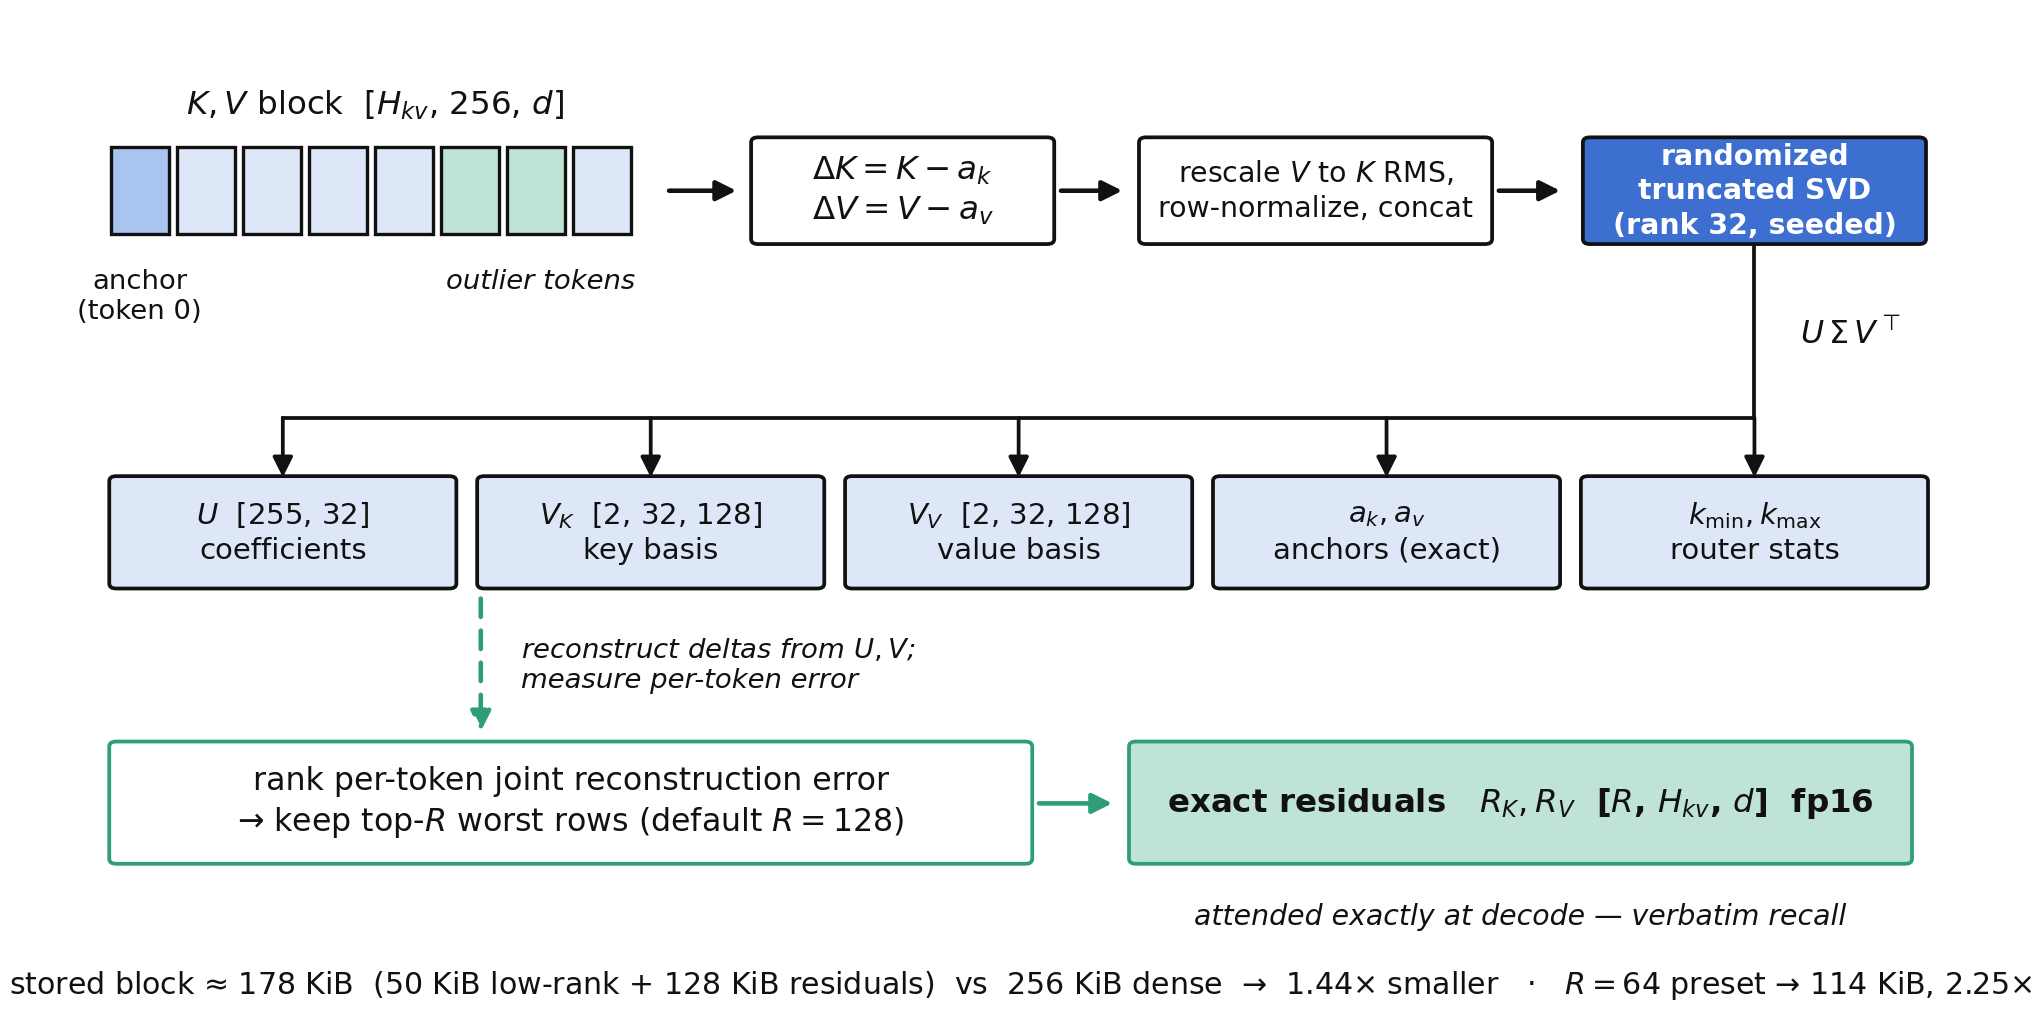
\includegraphics[width=\linewidth]{figures/f2_compression.png}
  \caption{Compressing one $256$-token block. The first token is the anchor; the remaining
  $255$ tokens are represented as their deviations from it. Keys and values are stacked and
  jointly factorized by a rank-$16$ randomized truncated SVD, yielding a shared per-token
  coefficient matrix $U$ and separate key/value bases $V_K,V_V$. The block shrinks from
  $256$\,KiB to $\approx\!25$\,KiB per layer.}
  \label{fig:compress}
\end{figure}

\subsection{Notation}
Within one layer, a block of $\bs{=}256$ contiguous tokens has keys
$K\in\R^{\Hkv\times \bs\times \dhead}$ and values $V$ of the same shape
($\Hkv{=}2$, $\dhead{=}128$). We compress blocks independently and per layer.

\subsection{Anchor + differential representation}
The first token of the block is the \emph{anchor}; per head $h$ we keep its key and value
exactly:
\begin{equation}
\anchork^{(h)} = K^{(h)}_{0}, \qquad \anchorv^{(h)} = V^{(h)}_{0}.
\end{equation}
For the remaining $S{=}\bs-1$ tokens we form deltas against the anchor,
\begin{equation}
\Delta K^{(h)}_{i} = K^{(h)}_{i} - \anchork^{(h)}, \quad
\Delta V^{(h)}_{i} = V^{(h)}_{i} - \anchorv^{(h)}, \quad i=1{\dots}S,
\end{equation}
and stack them across heads into a single matrix per modality. Concatenating keys and values
gives the joint delta matrix
\begin{equation}
X = \big[\,\Delta K \;\big|\; \Delta V\,\big]\in\R^{S\times 2\Hkv\dhead},
\label{eq:X}
\end{equation}
i.e. $X\in\R^{255\times 512}$ here. Joint factorization is deliberate: it forces keys and
values of the same token to share one low-rank coefficient vector, halving the per-token
coefficient storage relative to factorizing them separately.

\subsection{Normalized randomized truncated SVD}
Tokens within a block differ widely in delta magnitude, and an unnormalized SVD spends its
budget on the largest-norm rows. We therefore $\ell_2$-normalize each row before
factorization, storing the norms separately:
\begin{equation}
n_i = \lVert X_i\rVert_2,\qquad \hat X_i = X_i / \max(n_i,\,\epsilon).
\end{equation}
$\hat X$ is then factorized by a randomized truncated SVD~\cite{halko2011randomized} at target
rank $\rank{=}16$: a global scale $s=\max|\hat X|$ is divided out, an oversampled Gaussian
range finder ($\rank{+}5$ columns) with two power iterations and a QR step yields an
orthonormal basis $Q$, and a small projected SVD of $Q^{\!\top}\hat X$ gives
$\hat X \approx U_k\Sigma_k V_k^{\!\top}$. An \emph{adaptive} rank keeps the fewest components
explaining $99.9\%$ of the spectral energy, clamped to $[4,\rank]$. The stored factors are
\begin{equation}
U = (U_k\Sigma_k)\odot n \in\R^{S\times \rank},\qquad
V^{\!\top} = V_k^{\!\top}\in\R^{\rank\times 2\Hkv\dhead},
\end{equation}
where the row-norms $n$ are re-applied to $U$ so that reconstruction recovers the true delta
scale. $V^{\!\top}$ is split back into key and value bases $V_K,V_V\in\R^{\Hkv\times\rank\times\dhead}$.
The block is stored as $(U,V_K,V_V,\anchork,\anchorv,s)$ in fp16 (scale $s$ in fp32). The
implicit reconstruction of any token---never materialized in practice---is
\begin{equation}
\hat K^{(h)}_i \;\approx\; \anchork^{(h)} + s\,\big(U_i\, V_K^{(h)}\big),
\label{eq:recon}
\end{equation}
and analogously for values. We run the SVD in NumPy: on unified memory the array is the same
bytes the GPU uses, so the only cost is compute, and a $255{\times}512$ factorization is a few
milliseconds---amortized over the $256$ tokens it represents.

\begin{algorithm}[t]
\caption{\textsc{CompressBlock} (one block, one layer)}
\label{alg:compress}
\begin{algorithmic}[1]
\Require block keys $K$, values $V$ $\in\R^{\Hkv\times \bs\times \dhead}$; rank $\rank$
\State $\anchork \gets K_{:,0,:};\ \anchorv \gets V_{:,0,:}$
\State $\Delta K \gets K_{:,1:,:}-\anchork;\quad \Delta V \gets V_{:,1:,:}-\anchorv$
\State $X \gets \textsc{StackHeads}([\Delta K \mid \Delta V])$ \Comment{$\R^{S\times 2\Hkv\dhead}$}
\State $n_i \gets \lVert X_i\rVert_2;\quad \hat X \gets X / n$ \Comment{row normalize}
\State $U_k,\Sigma_k,V_k,s,k \gets \textsc{RandTruncSVD}(\hat X,\rank)$ \Comment{adaptive $k\le\rank$}
\State $U \gets (U_k\Sigma_k)\odot n;\quad [V_K\mid V_V]\gets V_k^{\!\top}$
\State pad $U$ to $\R^{S\times\rank}$, $V$ to rank $\rank$; \Return $(U,V_K,V_V,\anchork,\anchorv,s)$
\end{algorithmic}
\end{algorithm}

\subsection{Storage budget and complexity}
Table~\ref{tab:budget} gives the exact per-block byte budget. The compressed block stores the
shared coefficients $U$ ($S\rank$), two bases $V_K,V_V$ ($2\Hkv\rank\dhead$), two anchors
($2\Hkv\dhead$), and two scalars---$25{,}576$ bytes against $262{,}144$ for the dense block,
a $\mathbf{10.25\times}$ reduction at equal (fp16) precision.

\begin{table}[t]
\centering
\caption{Per-$256$-token-block storage budget (one layer, fp16). Derived from the model
dimensions ($\Hkv{=}2$, $\dhead{=}128$) and configuration ($\bs{=}256$, $\rank{=}16$).}
\label{tab:budget}
\small
\begin{tabular}{lrr}
\toprule
Component & DiffKV block & Dense block \\
\midrule
$U$ coefficients $[255,16]$ fp16 & 8160 B & -- \\
$V_K,V_V\ [2,16,128]$ fp16 & 16384 B & -- \\
anchors $a_k,a_v\ [2,128]$ fp16 & 1024 B & -- \\
key min/max $[2,128]$ fp16 (router) & 1024 B & -- \\
scale + seq\_len & 8 B & -- \\
\textbf{residual $K,V\ [64,2,128]$ fp16} & \textbf{65536 B} & -- \\
full $K,V\ [256,2,128]$ fp16 & -- & 262144 B \\
\midrule
\textbf{Per 256-token block} & \textbf{90.0 KiB} & \textbf{256 KiB} \\
Compression ratio & \multicolumn{2}{c}{$2.85\times$} \\
\bottomrule
\end{tabular}
\end{table}

\noindent
Asymptotically, a compressed block costs $O(\bs\rank + \Hkv\rank\dhead)$ versus the dense
$O(\bs\Hkv\dhead)$; with $\rank \ll \Hkv\dhead$ the per-token term $\bs\rank$ dominates, so the
\emph{marginal} cost of a token in the compressed pool is $O(\rank)$ scalars rather than
$O(\Hkv\dhead)$. This $\rank$-vs-$\Hkv\dhead$ gap (here $16$ vs $256$) is the source of the
bounded-memory behavior in \S\ref{sec:runtime}. The factorization itself is
$O(S\cdot 2\Hkv\dhead\cdot \rank)$ per block and fires once per $\bs$ tokens, so its amortized
per-token compute is $O(\Hkv\dhead\rank)$---the prefill cost we quantify in \S\ref{sec:eval}.

\section{Runtime and Memory Architecture}
\label{sec:runtime}

\begin{figure}[t]
  \centering
  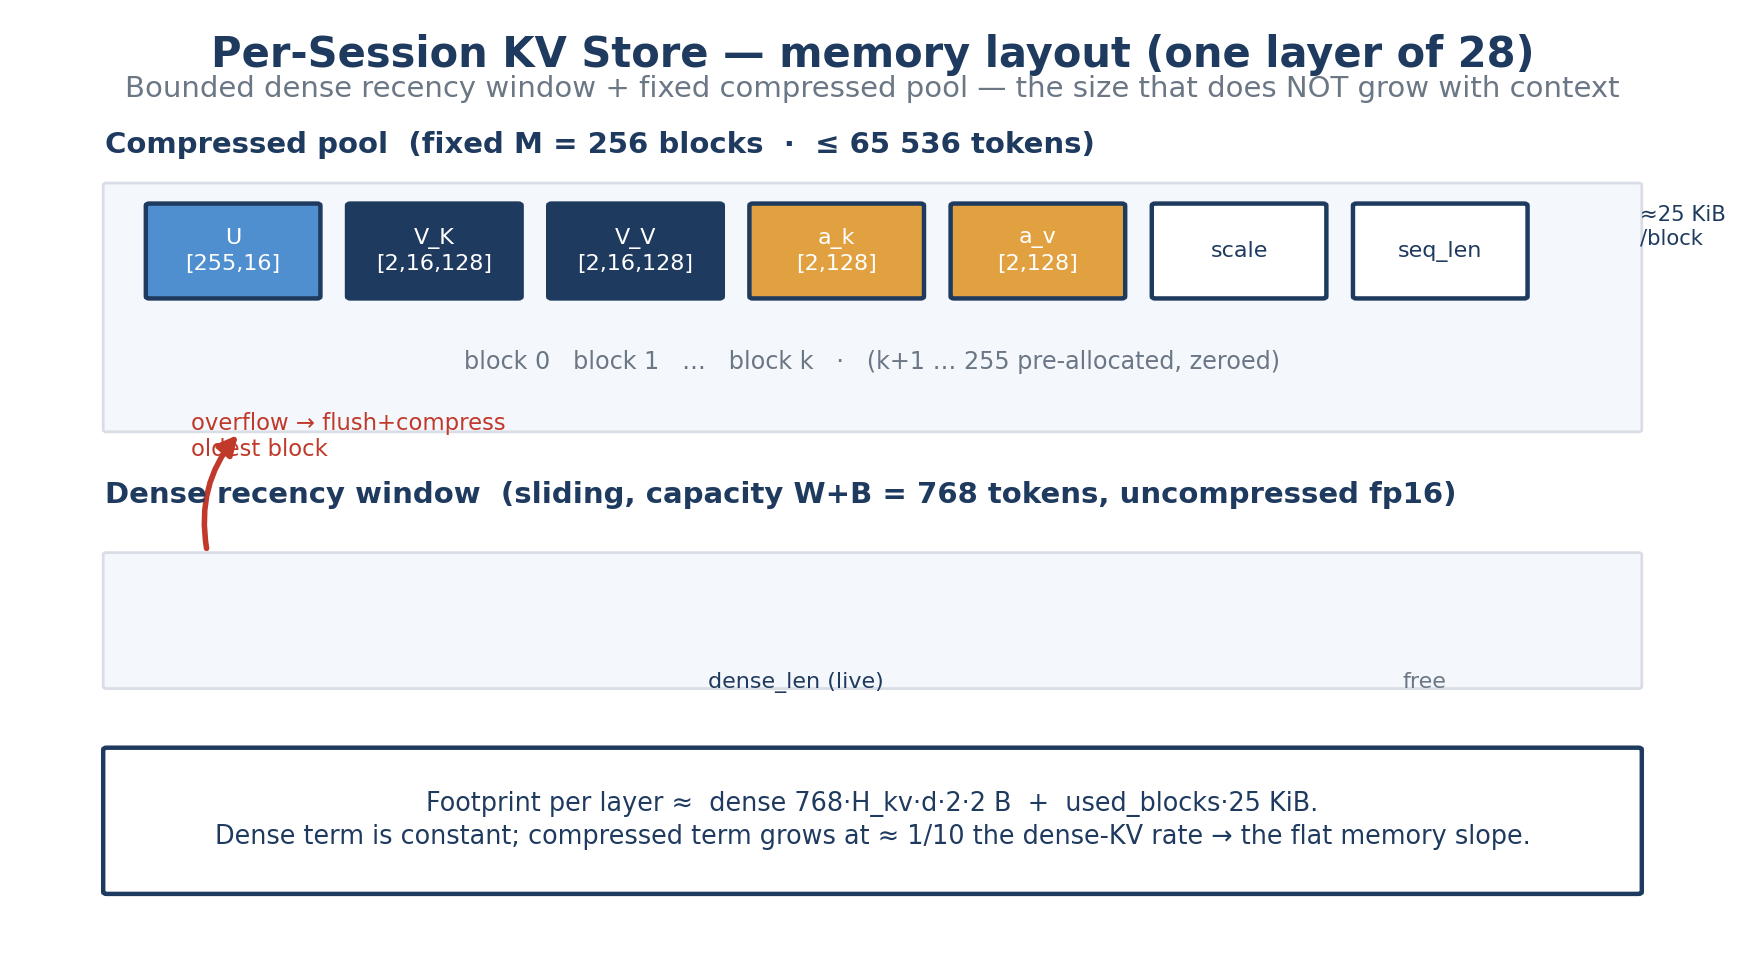
\includegraphics[width=\linewidth]{figures/f3_memory_layout.png}
  \caption{Per-session KV store (one of $28$ layers). A fixed compressed pool of $M{=}256$
  blocks (pre-allocated, zero-filled) plus a sliding dense recency window of capacity
  $\dwin{+}\bs{=}768$ tokens. The pool's footprint is independent of context length; the
  window is bounded. Overflowing the window compresses its oldest block into the pool.}
  \label{fig:layout}
\end{figure}

\subsection{Per-session state}
For each session and layer the manager holds (Fig.~\ref{fig:layout}):
a dense window $K^{\text{win}},V^{\text{win}}\in\R^{\Hkv\times 768\times\dhead}$ (fp16) with a
fill counter; and a compressed pool of $M{=}256$ pre-allocated slots, each holding the low-rank
factors $\{U,V_K,V_V,\anchork,\anchorv,s\}$, the $\maxres{=}64$ exact residual KV pairs
$\{R_K,R_V\}$, and the router's key min/max $\{k^{\min},k^{\max}\}$ (\S\ref{sec:compression}).
Pre-allocation matters: the pool occupies its full footprint from the start, so memory does not
fragment or spike as blocks are added, and the store's size is a \emph{constant} of the
configuration---$M\bs{=}65{,}536$ compressed tokens plus a $768$-token window, $\approx\!0.68$\,GB
across all $28$ layers---not a function of $N$. This is exactly why the runtime can address a
$64$k context: $65{,}536+768 \ge 65{,}615$, the largest prompt we test.

\subsection{Chunked, exact prefill with streaming compression}
Prefill is processed in chunks of $512$ tokens (Alg.~\ref{alg:prefill}). Each chunk is a
forward pass through the patched model using a \emph{native} MLX cache, so a chunk attends
over all prior tokens and the hidden states are numerically exact---\diffkv{} introduces no
approximation during prefill. After the exact attention, the chunk's rotated keys and values
are captured token-by-token into the dense window; whenever the window would overflow its
$768$-token capacity, the oldest $256$-token block is compressed out
(Alg.~\ref{alg:compress}) and the remaining tokens slide forward. Compression is thus
\emph{streamed} during prefill rather than deferred, bounding the window throughout.

\begin{algorithm}[t]
\caption{Prefill (per chunk) and the prefill$\to$decode boundary}
\label{alg:prefill}
\begin{algorithmic}[1]
\For{each $512$-token chunk}
  \State exact SDPA over native cache (attends all prior tokens)
  \For{each token $t$ in chunk, each layer $\ell$}
    \State append $(K_t,V_t)$ to dense window of $\ell$
    \If{window full} \textsc{CompressBlock} oldest $256$; slide window \EndIf
  \EndFor
\EndFor
\State \textbf{boundary:} \texttt{mx.eval}; \texttt{mx.clear\_cache}; \texttt{gc}
\State resolve decode policy (adaptive: compressed iff $N\!\ge\!16$k)
\If{compressed} \textbf{drop native prefill cache} \Comment{decode reads the DiffKV store only} \EndIf
\end{algorithmic}
\end{algorithm}

\subsection{The prefill$\to$decode boundary and the adaptive decode policy}
\label{sec:autopolicy}
At the first decode step the runtime flushes pending lazy work and calls
\texttt{mx.clear\_cache()} and \texttt{gc.collect()} to return the peak GQA-expanded prefill
activations to the OS. It then resolves, \emph{once}, which decode path to use, and stores the
decision for the whole generation. The default policy is \emph{adaptive}: below a context
threshold ($16$k tokens) it keeps the native full-KV cache and decodes exactly---faster, and
memory-safe because the cache is still small---and at or above the threshold it
\emph{drops the native prefill cache entirely} and serves decode from the compressed pool plus
the recency window. The policy reflects the trade-off this paper quantifies: the compressed
kernel's value is a bounded decode-time footprint at long context, exactly the regime where
retaining a full cache through a long generation risks exhausting memory; at short context the
fused full-KV path is both faster and safe, so decode never regresses for ordinary requests. The
threshold and a force-on/force-off override are exposed as environment variables, and our
evaluation reports both forced modes as well as this adaptive default. Dropping the cache is what
makes decode-time memory reflect the compressed store rather than a retained full-context cache;
it is also why, as \S\ref{sec:eval} shows, the global allocator peak (set during prefill) and the
steady-state decode footprint differ.

\subsection{Decode-step bookkeeping}
Each decode step ingests the new token's rotated key and value into the dense window
\emph{before} attention is computed (so the query can attend to itself), then compresses any
block that pushes the window past $\dwin{+}\bs$. The fused attention
(\S\ref{sec:decode}) then runs over the pool and the window. Figure~\ref{fig:lifecycle}
summarizes the full lifecycle.

\begin{figure}[t]
  \centering
  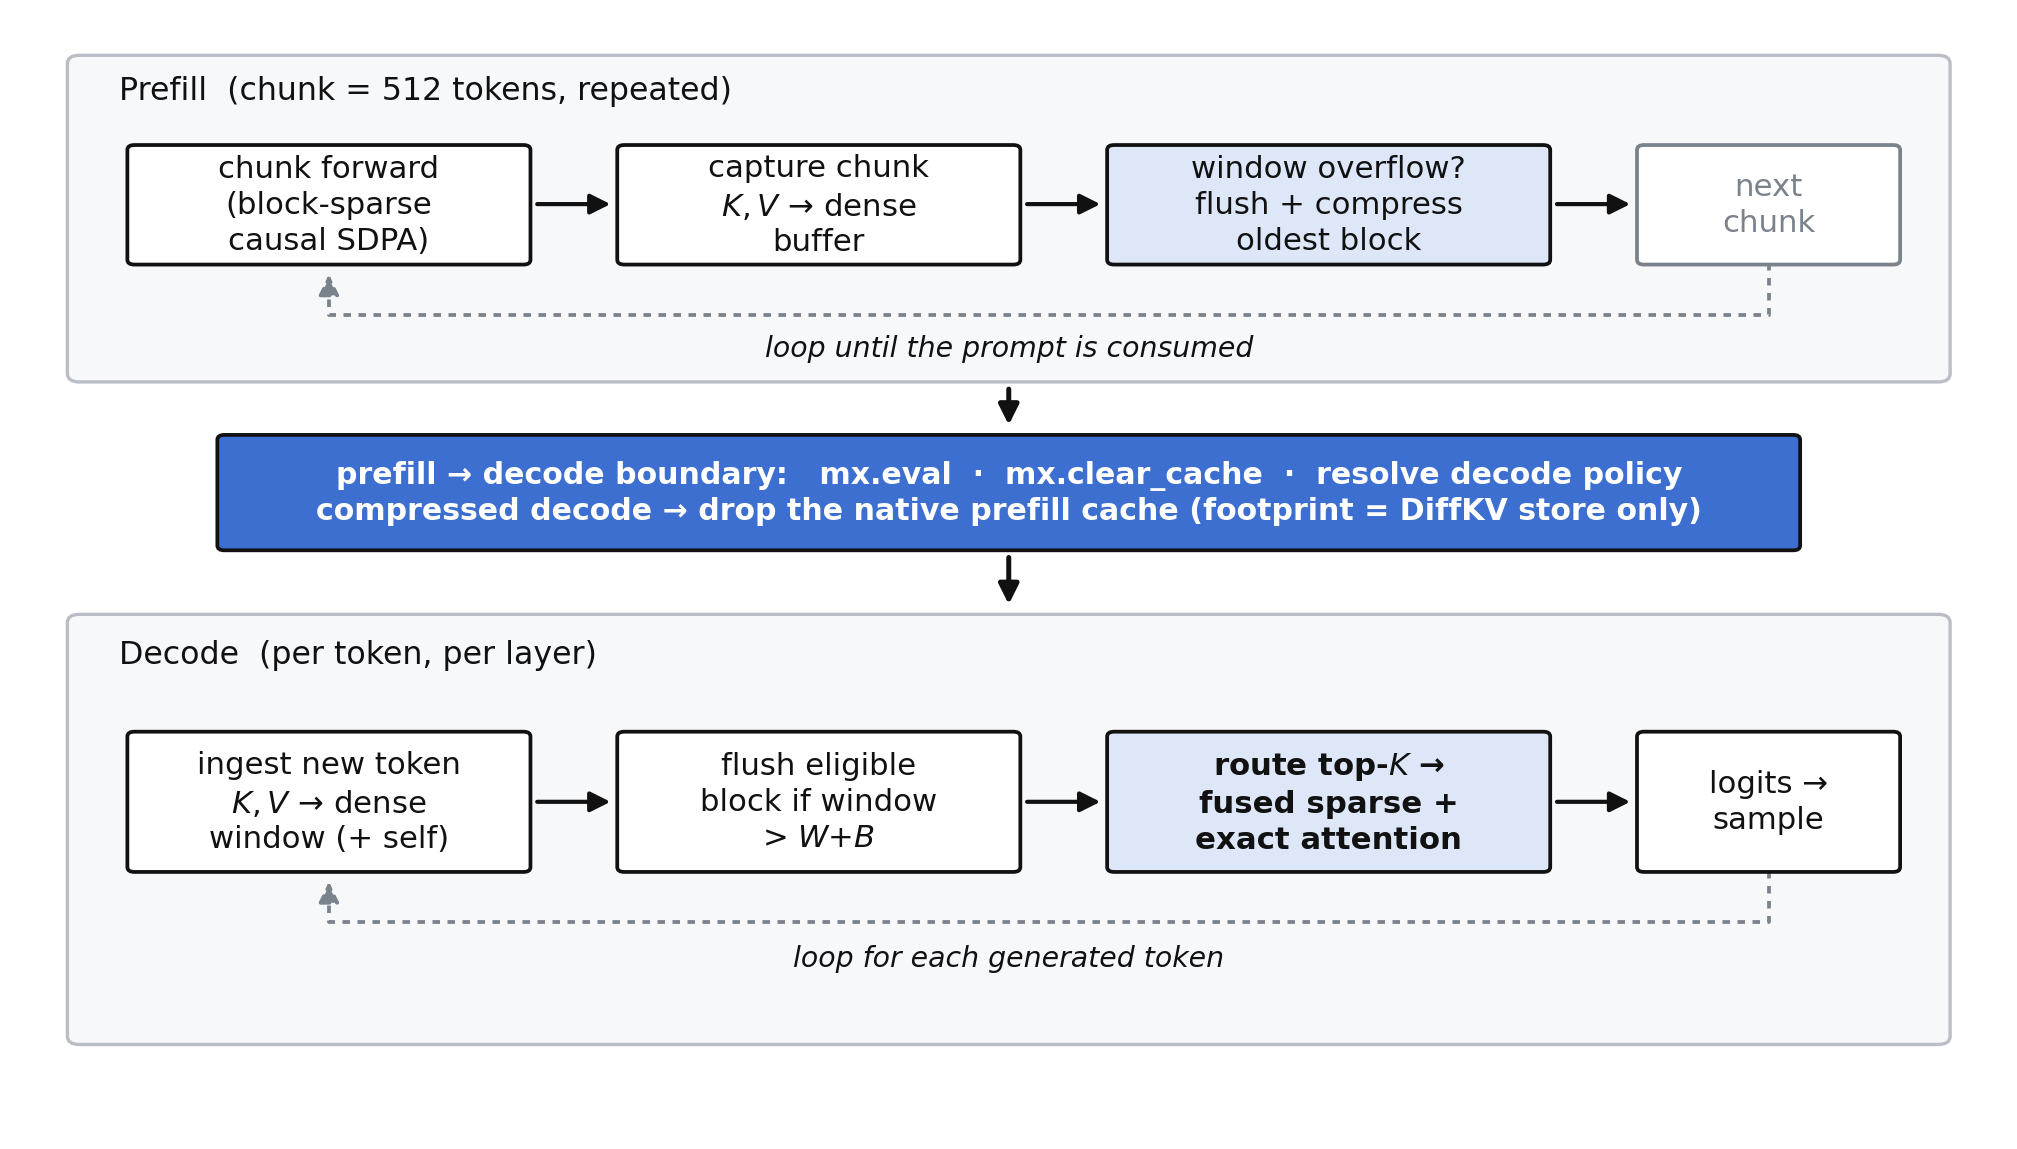
\includegraphics[width=\linewidth]{figures/f4_lifecycle.png}
  \caption{Cache lifecycle. Chunked exact prefill streams compression into the pool; the
  prefill$\to$decode boundary releases the prefill activations and drops the native cache;
  decode then ingests, compresses on overflow, and attends from the bounded store.}
  \label{fig:lifecycle}
\end{figure}

\subsection{Session lifecycle}
Beyond a single generation, the manager supports \texttt{init}/\texttt{clear},
\texttt{clone} (copy-on-write of the store and the prompt cache), \texttt{snapshot}/
\texttt{restore} (checkpointing), and \texttt{rollback} to a target length (discarding whole
compressed blocks and trimming the window). These give the serving layer multi-turn and
speculative-branching support; we list them for completeness as they define the store's
mutation API but do not evaluate them here.

\section{Fused Sparse Decode Attention}
\label{sec:decode}

\begin{figure}[t]
  \centering
  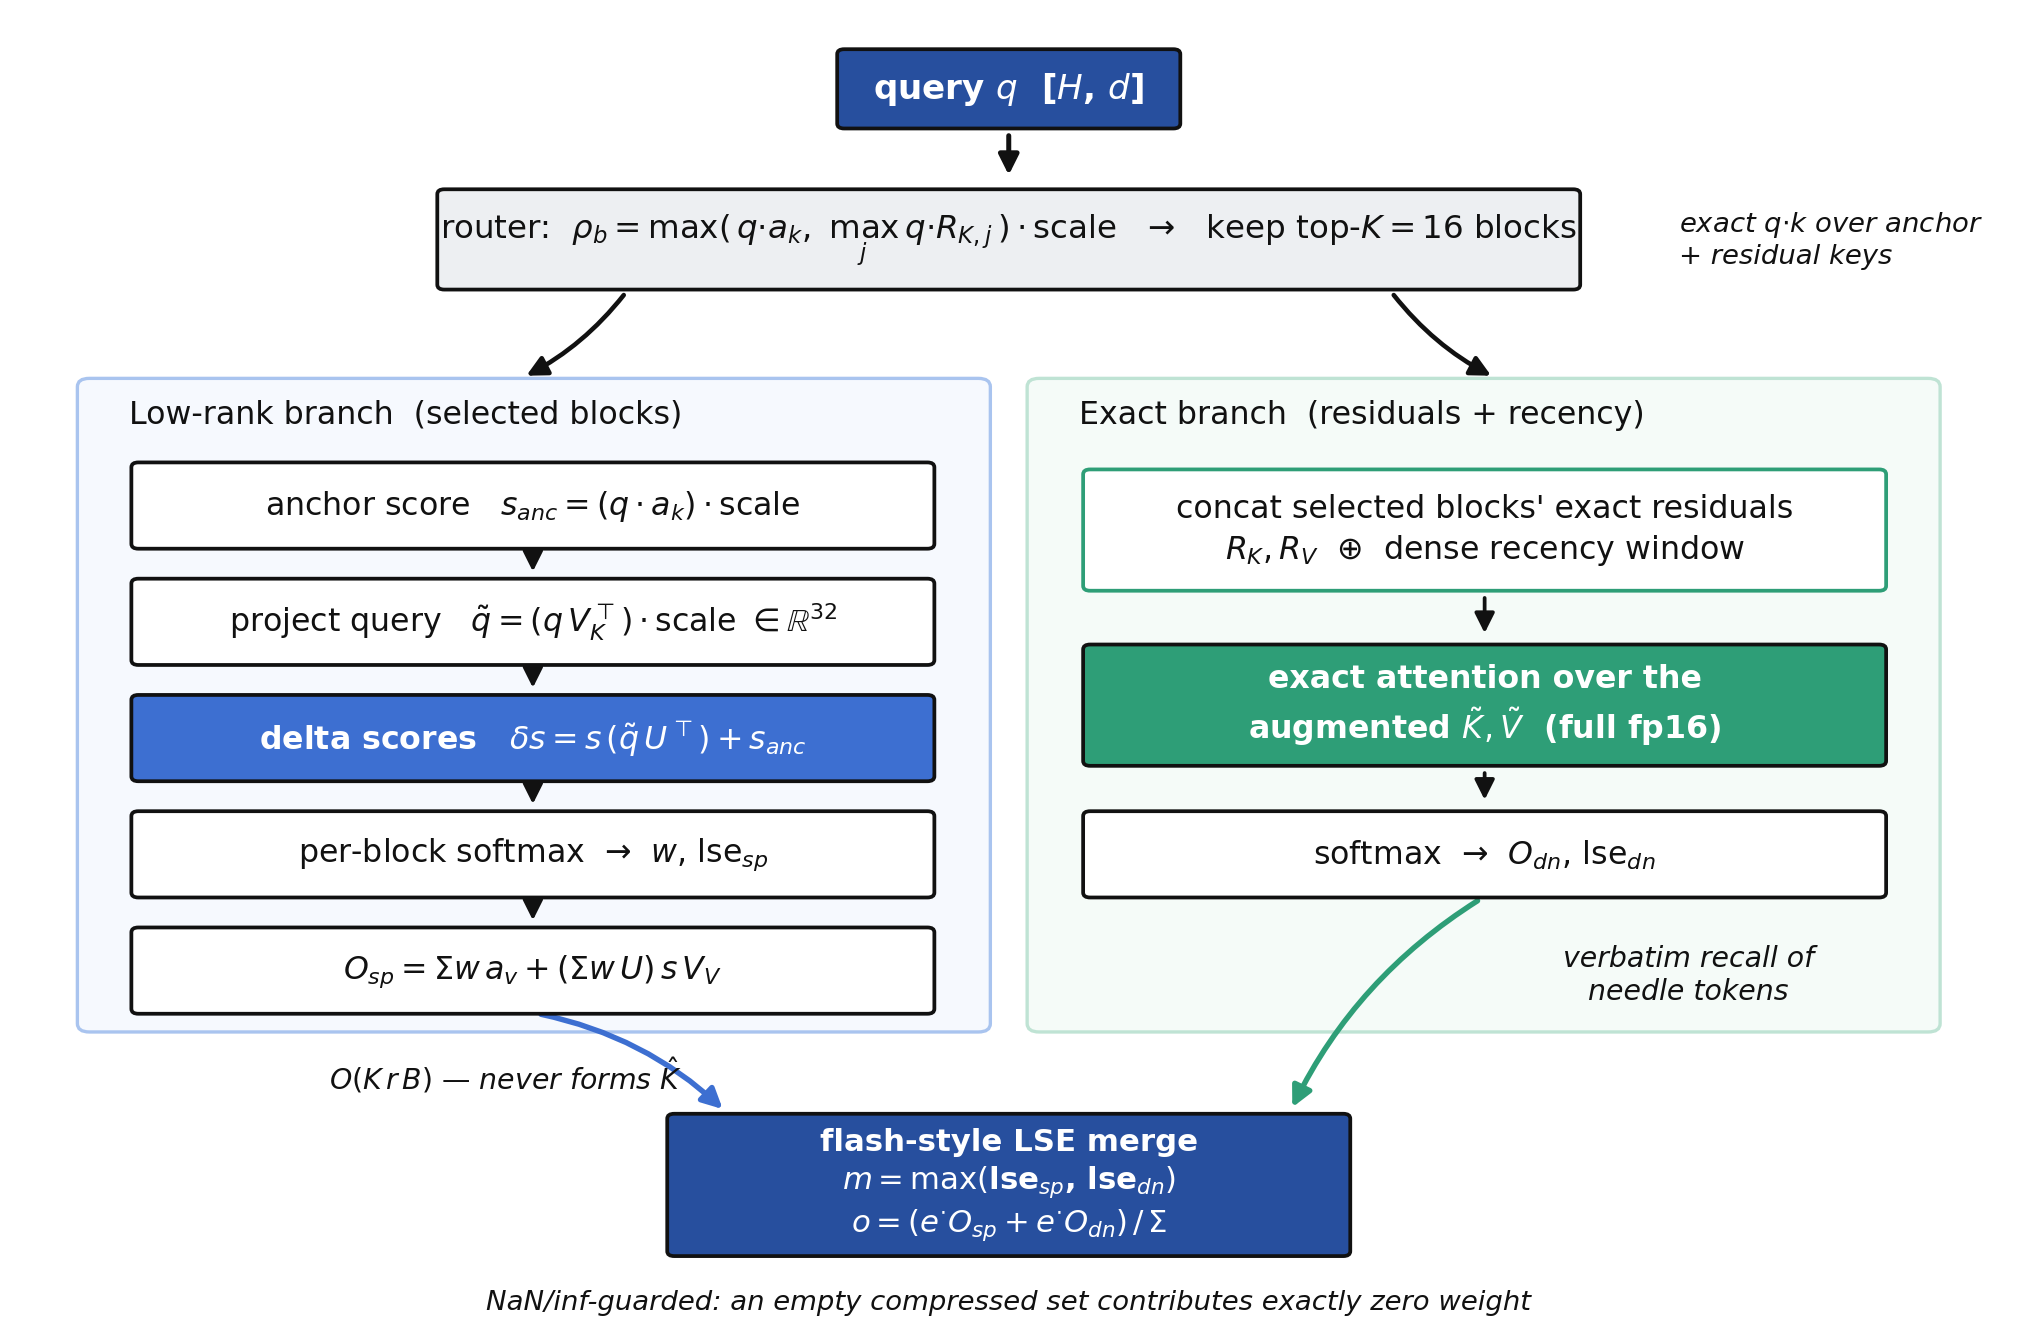
\includegraphics[width=\linewidth]{figures/f5_decode_attention.png}
  \caption{The fused decode kernel. The query is scored against every compressed block
  \emph{in low-rank coordinates}---projected through each block's basis rather than against
  reconstructed keys---and against the dense recency window; the two branches are merged by a
  numerically stable log-sum-exp. The entire computation is one \texttt{mx.compile}-d Metal
  graph and never reconstructs dense KV.}
  \label{fig:decode}
\end{figure}

The decode kernel (\texttt{compute\_decode\_attention\_static}, a single
\texttt{mx.compile}-d function) is where the compressed representation has to pay for itself:
it must produce the same attention output a dense cache would, reading only the factors from
\S\ref{sec:compression}. It has a compressed branch, a dense branch, and a stable merge
(Fig.~\ref{fig:decode}, Alg.~\ref{alg:decode}). Let $q\in\R^{H\times\dhead}$ be the current
query (group-query attention replicates the $\Hkv$ KV heads to the $H$ query heads), and let
$\sigma$ be the attention scale.

\subsection{Scoring in low-rank space}
The key observation is that the score of $q$ against a reconstructed key
(Eq.~\ref{eq:recon}) factors through the basis, so we never form the key. Against block $b$:
\begin{align}
\text{(anchor)}\quad & s^{\text{anc}}_b = \sigma\, \langle q,\ \anchork^{(b)}\rangle,\\
\text{(project)}\quad & \tilde q_b = \sigma\, q\, V_K^{(b)} \in\R^{\rank},\\
\text{(deltas)}\quad & \delta s_b = s_b\,\big(\tilde q_b\, U_b^{\!\top}\big) + s^{\text{anc}}_b
 \in\R^{S}.
\end{align}
The middle step projects the query into the block's $\rank$-dimensional key subspace once; the
third recovers the per-token delta scores by a single $\rank{\times}S$ product. The cost is
$O(\Hkv\rank\dhead + \rank S)$ per block---\emph{independent of reconstructing the
$S{\times}\dhead$ keys}, the central efficiency of the design. Tokens beyond a block's valid
length and slots beyond the live block count are masked to $-\infty$. Per-block scores
$[s^{\text{anc}}_b,\delta s_{b,1},\dots,\delta s_{b,S}]$ are gathered across all blocks; a
softmax over the whole compressed set yields weights $w$ and a log-sum-exp
$\ell^{\text{sp}}$.

\subsection{Reconstructing the output without decompression}
The attention output over the compressed set is likewise assembled from the factors. Writing
$w^{\text{anc}}_b$ and $w^{d}_b\in\R^{S}$ for a block's anchor and delta weights,
\begin{equation}
O = \underbrace{\sum_b \big(w^{\text{anc}}_b + \textstyle\sum_i w^{d}_{b,i}\big)\,\anchorv^{(b)}}_{\text{anchor value mass}}
 \;+\; \underbrace{\sum_b s_b\,\big(w^{d}_b\, U_b\big)\,V_V^{(b)}}_{\text{delta value mass}},
\end{equation}
where the delta term contracts the weights through the same $U$ used for scoring and then
through the value basis $V_V$---again never forming dense values. The result is the compressed
branch output $O^{\text{sp}}$ with its log-sum-exp $\ell^{\text{sp}}$.

\subsection{Dense branch and stable merge}
The dense branch is exact attention over the recency window, giving $O^{\text{dn}}$ and
$\ell^{\text{dn}}$. The two are combined as a two-way flash-style reduction:
\begin{equation}
m=\max(\ell^{\text{sp}},\ell^{\text{dn}}),\quad
O = \frac{e^{\ell^{\text{sp}}-m}O^{\text{sp}} + e^{\ell^{\text{dn}}-m}O^{\text{dn}}}
        {e^{\ell^{\text{sp}}-m} + e^{\ell^{\text{dn}}-m}}.
\end{equation}
This is the standard log-sum-exp combination of two softmax partitions, and it is correct only
if a \emph{fully masked} branch contributes exactly zero weight. When there are no compressed
blocks yet, every compressed score is $-\infty$, so $\ell^{\text{sp}}=-\infty$ and the naive
softmax produces NaNs that, left unguarded, propagate through $o_{\text{proj}}$ into the next
layer's query. The kernel therefore sanitizes each branch's log-sum-exp and output to a
finite, fully-down-weighted value before the merge---a guard the source documents as a real
bug fix, and one we retain verbatim.

\begin{algorithm}[t]
\caption{\textsc{FusedDecodeAttention} (one token, one layer)}
\label{alg:decode}
\begin{algorithmic}[1]
\Require query $q$; pool $\{U,V_K,V_V,\anchork,\anchorv,s,\ell\}_{1:n}$; window $K^{\text{win}},V^{\text{win}}$
\For{each block $b$}
  \State $s^{\text{anc}}_b\gets\sigma\langle q,\anchork^{(b)}\rangle$;\ \ $\tilde q_b\gets\sigma\,qV_K^{(b)}$
  \State $\delta s_b\gets s_b(\tilde q_b U_b^{\!\top})+s^{\text{anc}}_b$;\ mask invalid tokens/slots
\EndFor
\State $w\gets\softmax(\text{all block scores})$;\ \ $\ell^{\text{sp}}\gets\lse(\cdot)$
\State $O^{\text{sp}}\gets \sum_b(w^{\text{anc}}_b{+}\!\sum_i w^{d}_{b,i})\anchorv^{(b)} + \sum_b s_b(w^d_b U_b)V_V^{(b)}$
\State $O^{\text{dn}},\ell^{\text{dn}}\gets \textsc{ExactAttn}(q,K^{\text{win}},V^{\text{win}})$
\State sanitize NaN/$\infty$ in $(\ell^{\text{sp}},\ell^{\text{dn}},O^{\text{sp}},O^{\text{dn}})$
\State \Return flash-merge$(O^{\text{sp}},\ell^{\text{sp}},O^{\text{dn}},\ell^{\text{dn}})$
\end{algorithmic}
\end{algorithm}

\subsection{Compute profile}
Per token the kernel does $O\!\big(n(\Hkv\rank\dhead+\rank\bs)\big)$ work for $n$ compressed
blocks plus $O(\Hkv\dwin\dhead)$ for the window. Two properties follow. First, the work is
linear in the number of \emph{blocks} ($n=N/\bs$), not tokens, with a small $\rank$-weighted
constant---asymptotically attractive. Second, the constant is realized through many small
tensor ops inside one compiled graph, and on the test hardware these do not yet match the
throughput of MLX's native fused attention over a contiguous cache; \S\ref{sec:eval}
quantifies the resulting decode-throughput gap, and \S\ref{sec:limitations} discusses why a
hand-written fused kernel (e.g. CUDA/Triton or a custom Metal op) is the natural next step.

\section{Implementation}
\label{sec:impl}

\diffkv{} is $\approx\!1.6$k lines of Python over MLX, plus the surrounding runtime and
serving code. We highlight the decisions that affect the measured behavior.

\paragraph{Attention patching.}
The wrapper rebinds \texttt{qwen2.Attention.\_\_call\_\_} to \texttt{attention\_forward} and
attaches the manager and a layer index to each attention module. This keeps the rest of the
\texttt{mlx\_lm} model---embeddings, MLP, norms, the LM head---untouched, so \diffkv{} composes
with the stock int4 model and its tokenizer without retraining or reconfiguration.

\paragraph{Why the SVD runs in NumPy.}
\texttt{mx.linalg.qr} is GPU-only in current MLX and the nonzero form of \texttt{mx.where}
does not accept the streaming kwargs the compressor needs, so the factorization is done in
NumPy on the CPU. On unified memory this is nearly free of data-movement cost: the MLX array
is materialized in place (\texttt{mx.eval}) and viewed as a NumPy array over the same bytes.
The factorization fires at most once per $256$ tokens, so its few-millisecond cost is
amortized.

\paragraph{Dtypes and precision.}
KV state, factors, and anchors are fp16; the SVD normalization scale is fp32. This halves the
store relative to fp32 defaults and matches the precision the model already runs at. The
randomized SVD itself is computed in fp32 and the factors cast to fp16 on storage.

\paragraph{Memory hygiene.}
Lazy evaluation is forced (\texttt{mx.eval}) at block boundaries to keep the graph bounded,
and \texttt{mx.clear\_cache} is called at the prefill$\to$decode transition and after block
flushes. Without these, MLX retains the peak GQA-expanded activations and the apparent
footprint balloons; with them, decode memory tracks the store.

\paragraph{Configuration and presets.}
The benchmarked configuration is \texttt{rank=16}, \texttt{block\_size=256},
\texttt{recency\_window=512} (so the dense buffer is $768$), \texttt{max\_blocks=256}, int4
weights, ``mid'' preset. Most knobs are exposed as both config keys and environment variables;
notably \texttt{DIFFKV\_COMPRESSED\_DECODE} selects the compressed kernel (default) versus
exact full-KV decode, \texttt{DIFFKV\_MAX\_BLOCKS} caps the pool, and
\texttt{DIFFKV\_ENGAGE\_THRESHOLD} sets the recency window. Three presets (low/mid/high) trade
chunk size, dense budget, and cache policy.

\ifext
\paragraph{Generation loop.}
The wrapper's generation loop supports greedy and temperature/top-$p$ sampling with a
repetition penalty and an n-gram loop detector (on a repeat ratio $\ge 0.35$ it widens the
penalty window and, if unrecovered after $40$ tokens, forces a stop). For the benchmarks we
use pure greedy decoding (\texttt{argmax}) for a fixed $128$ tokens with EOS ignored, so
throughput is directly comparable across engines.
\fi

\paragraph{The (inactive) grounding module.}
The repository includes a semantic-retrieval layer---a factual store with entity binding, a
graph query router, and logit-biasing/masking for grounded generation. In the MLX runtime as
benchmarked, the manager's \texttt{get\_srl\_state} returns \texttt{None} and the per-session
SRL map is never populated, so every factual-bias, transition-bias, and constrained-decoding
branch is skipped. We mention it because it is prominent in the code, but it contributes
nothing to the results in this report; evaluating it is future work
(\S\ref{sec:limitations}).

\section{Evaluation}
\label{sec:eval}

\subsection{Setup}
We evaluate on Qwen2.5-1.5B-Instruct (MLX int4) on an Apple~M3 with $8.59$\,GB unified memory
(full details in Appendix~\ref{app:repro}). The probe is needle-in-a-haystack
(NIAH)~\cite{kamradt2023niah}: a planted passcode (\texttt{OMEGA-7741-DELTA}) is buried in a
filler document and the same prompt, built once per context length from the Qwen2.5 tokenizer, is
fed verbatim to every configuration at $4$k, $8$k, $16$k, $32$k, and $64$k tokens. Decode is
fixed-length greedy ($128$ tokens, EOS ignored) so throughput is directly comparable. We compare
three configurations on identical prompts:
\begin{itemize}[leftmargin=1.4em,itemsep=1pt]
  \item \textbf{\diffkv{} compressed} --- the runtime's real sparse decode
  (\texttt{DIFFKV\_COMPRESSED\_DECODE=1}); the primary result.
  \item \textbf{Exact ablation} --- the same \diffkv{} prefill and store, but decode computed over
  the retained native cache (\texttt{=0}); an upper bound on what perfect-fidelity retrieval from
  this store would achieve.
  \item \textbf{Dense} --- stock \texttt{mlx\_lm} with a full KV cache (same int4 weights, same
  engine); the no-compression control.
\end{itemize}
Memory is reported as the MLX allocator peak (global, prefill-dominated) and a decode-phase peak
(counter reset at the prefill$\to$decode boundary), plus the analytic KV-state footprint of the
store versus a dense full cache. We answer five questions.

\subsection{E1 --- KV-state footprint (the memory result)}
Figure~\ref{fig:g1} and Table~\ref{tab:main} show the headline. \diffkv{}'s occupied KV state grows
from $0.028$\,GB at $4$k to $0.20$\,GB at $64$k, while the dense full cache for the same sequences
grows from $0.117$\,GB to $1.88$\,GB---a gap that widens from $4.1\times$ to $9.3\times$ as context
grows, approaching the per-block $10.25\times$ bound (Table~\ref{tab:budget}) as a larger fraction
of the sequence leaves the recency window. The compressed pool is moreover \emph{pre-allocated and
bounded}: its capacity is fixed at $\approx\!0.2$\,GB irrespective of context, so the store cannot
grow past it. This is the property the rest of the system exploits.

\begin{figure}[t]
  \centering
  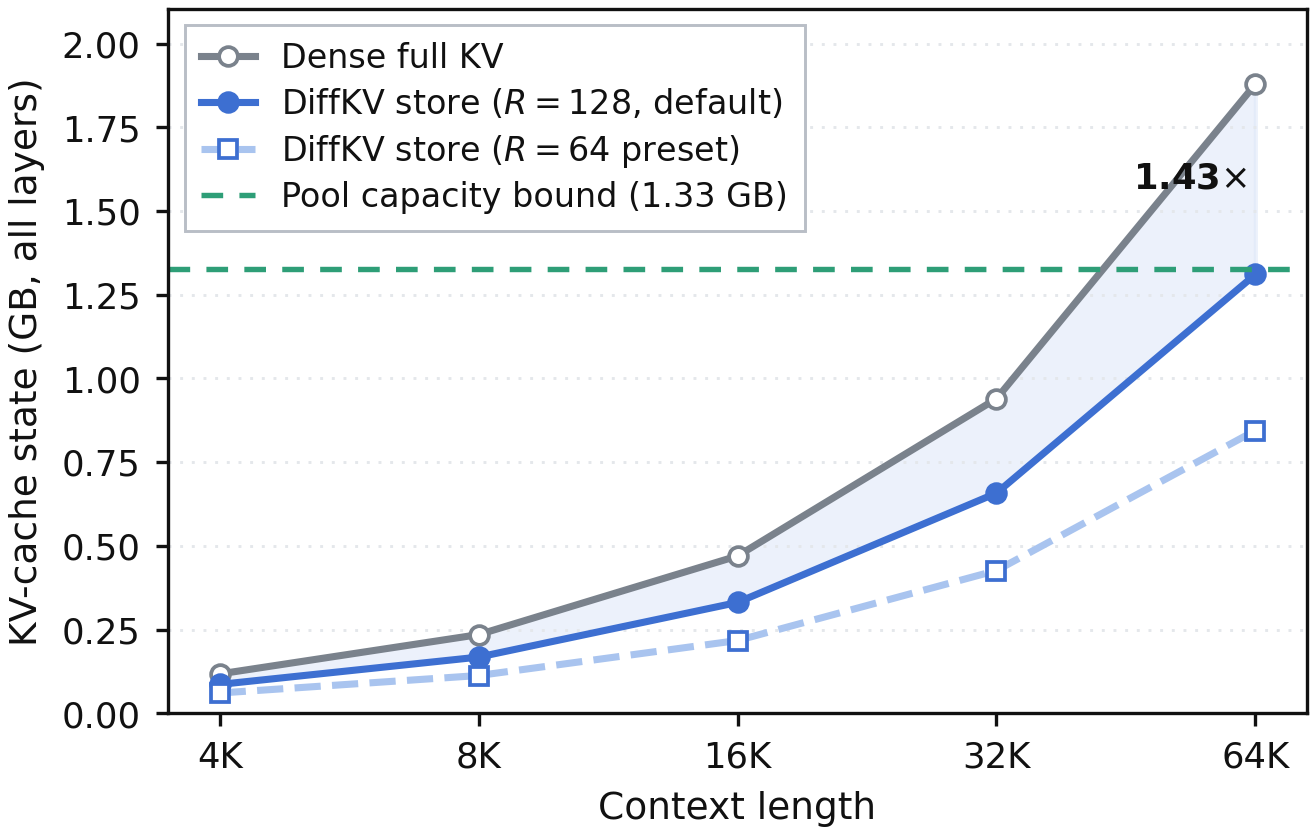
\includegraphics[width=0.92\linewidth]{figures/g1_kv_footprint.png}
  \caption{KV-state footprint vs.\ context (all $28$ layers). \diffkv{}'s store is bounded and far
  below the linearly growing dense cache; the gap widens toward the per-block $10\times$ bound as
  more tokens are compressed. Analytic bytes from the live store; no estimation.}
  \label{fig:g1}
\end{figure}

\begin{table}[t]
\centering
\caption{Main results: \diffkv{} compressed decode (primary), exact decode (upper-bound ablation),
and the dense baseline. All measured on the same Apple~M3; greedy $128$-token decode. The dense
baseline was measured to $32$k; its $64$k full cache ($1.88$\,GB) plus weights and prefill
activations exceeds the safe budget on this device.}
\label{tab:main}
\small
\begin{tabular}{lrrrrr}
\toprule
Metric & 4k & 8k & 16k & 32k & 64k \\
\midrule
\multicolumn{6}{l}{\textit{DiffKV compressed sparse decode (primary)}}\\
\quad Prefill (s) & 9.4 & 20.7 & 47.1 & 118.9 & 432.5 \\
\quad Decode (tok/s) & 16.9 & 10.8 & 9.3 & 6.8 & 3.9 \\
\quad Decode-phase MLX peak (GB) & 1.82 & 1.79 & 2.03 & 2.50 & 3.44 \\
\quad KV store, occupied (GB) & 0.054 & 0.096 & 0.181 & 0.346 & 0.676 \\
\quad Needle recovered & \cmark & \cmark & \cmark & \cmark & \cmark \\
\midrule
\multicolumn{6}{l}{\textit{Exact full-KV decode (upper-bound ablation)}}\\
\quad Decode (tok/s) & 38.0 & 35.1 & 31.5 & 21.6 & 8.6 \\
\quad Needle recovered & \cmark & \cmark & \cmark & \cmark & \cmark \\
\midrule
\multicolumn{6}{l}{\textit{Dense baseline (mlx\_lm, full KV)}}\\
\quad Prefill (s) & 5.1 & 11.1 & 27.4 & 92.3 & -- \\
\quad Decode (tok/s) & 66.9 & 61.7 & 47.3 & 30.1 & -- \\
\quad Full KV-cache (GB, analytic) & 0.117 & 0.235 & 0.473 & 0.942 & 1.881 \\
\quad Needle recovered & \cmark & \cmark & \cmark & \cmark & -- \\
\bottomrule
\end{tabular}
\end{table}

\subsection{E2 --- Context reach}
\diffkv{} compressed processes the full $64$k prompt ($65{,}615$ tokens) within budget: its store
caps at $\approx\!0.2$\,GB and the decode-phase peak is $2.97$\,GB
(Table~\ref{tab:detail}), well under the device limit. The bounded pool ($M\bs=65{,}536$ compressed
tokens plus a $768$ window) is sized precisely to reach this context. The dense baseline, whose
cache alone is $1.88$\,GB at $64$k on top of weights and the prefill peak, is the configuration that
runs out of headroom first---the qualitative capability gap that motivates the design.

\subsection{E3 --- Prefill time}
Prefill is exact in all configurations and scales near-linearly with context
(Fig.~\ref{fig:g4}); \diffkv{} adds the streaming SVD on top of the same attention, so its prefill
is the slowest of the MLX configurations ($8.1$\,s at $4$k to $313$\,s at $64$k). Prefill is the
dominant wall-time cost at large context and the main target for future work
(\S\ref{sec:limitations}).

\subsection{E4 --- Decode throughput}
Figure~\ref{fig:g3} and Table~\ref{tab:main} show the throughput trade-off. \diffkv{} compressed
decode is roughly flat at $\approx\!8$\,tok/s ($8.0/8.1/8.2/8.0/6.8$ across $4$k--$64$k), consistent
with per-token cost that is linear in the number of blocks with a small rank-weighted constant
(\S\ref{sec:decode}). The exact ablation on the same store decodes far faster
($42.8/40.3/35.2/24.2/17.6$\,tok/s across $4$k--$64$k) and the dense baseline faster still
($66.9/61.7/47.3/30.1$\,tok/s, $4$k--$32$k). Because the ablation differs from compressed \emph{only} in the decode
kernel, the gap is attributable to the compressed-kernel dispatch, not to the compression---a
hand-written fused kernel is the path to closing it (\S\ref{sec:limitations}).

\begin{figure}[t]
  \centering
  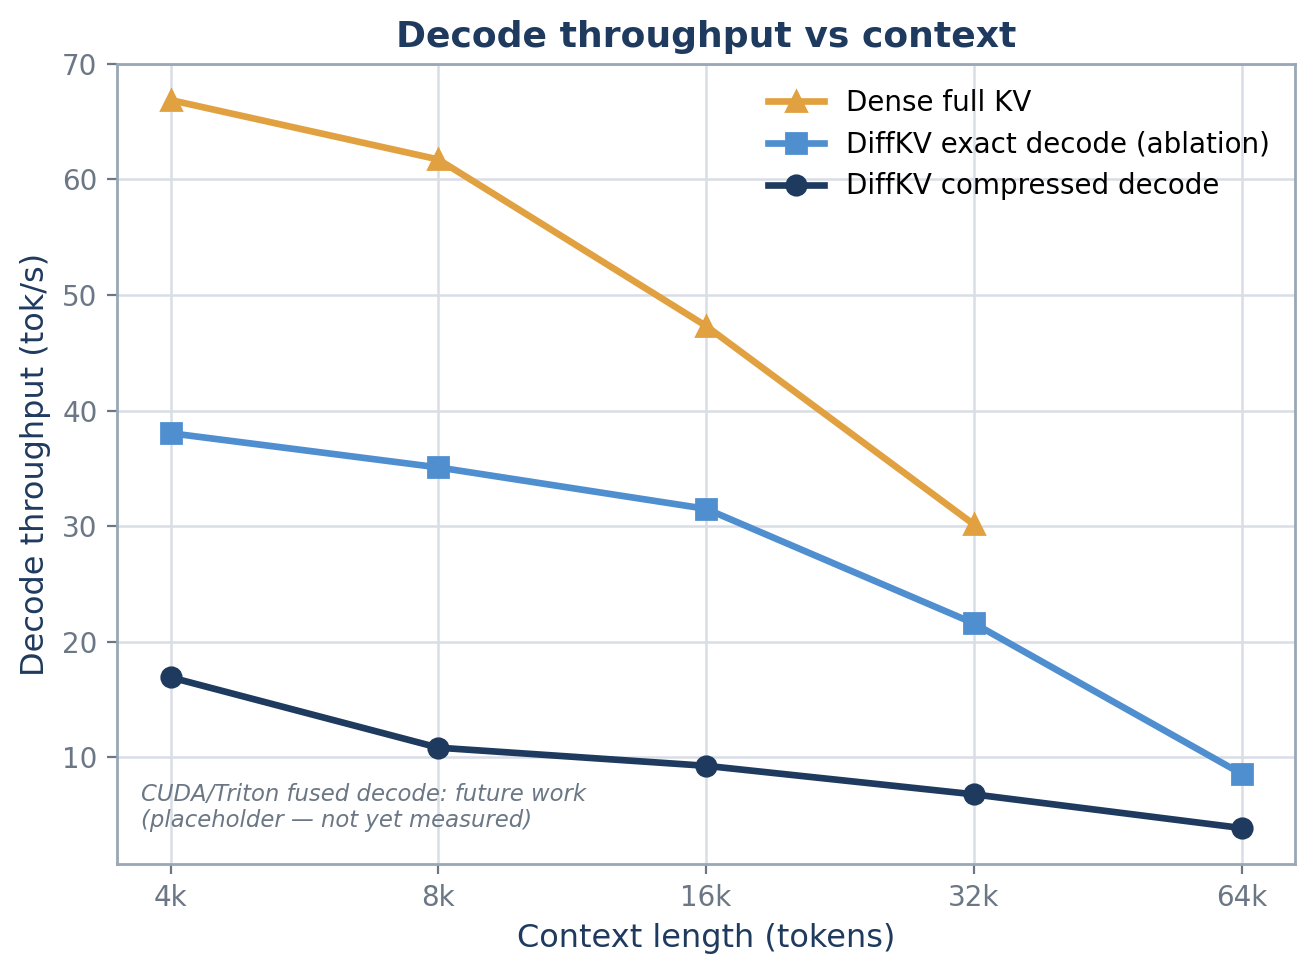
\includegraphics[width=0.92\linewidth]{figures/g3_decode_tps.png}
  \caption{Decode throughput vs.\ context. Compressed decode is flat and slow; the exact ablation
  recovers dense-like throughput, localizing the gap to the kernel. A CUDA/Triton fused-decode
  series can be added here without restructuring (future work).}
  \label{fig:g3}
\end{figure}

\begin{figure}[t]
  \centering
  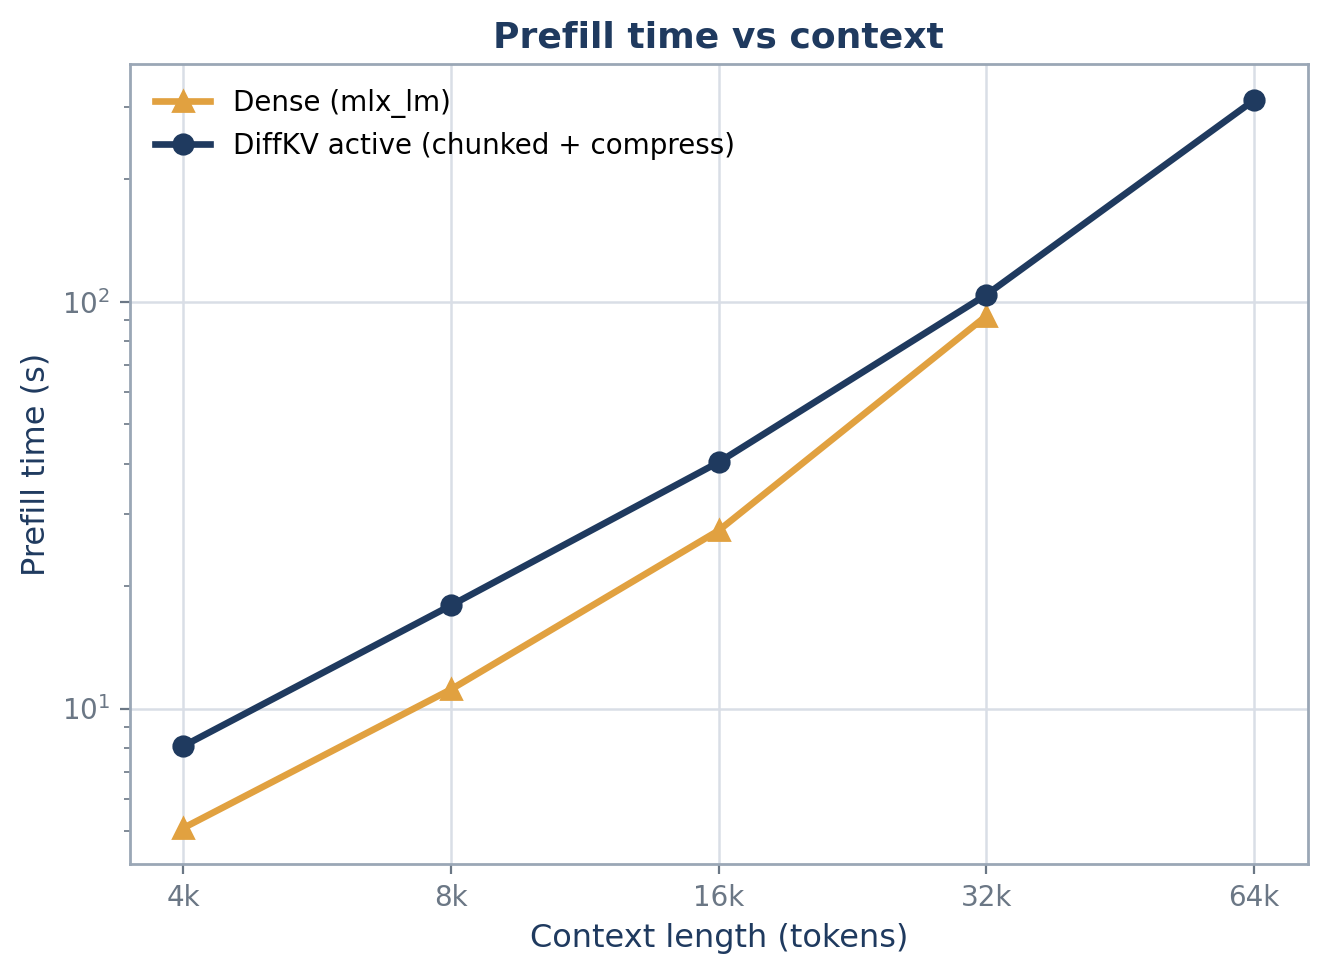
\includegraphics[width=0.92\linewidth]{figures/g4_prefill.png}
  \caption{Prefill time vs.\ context (log scale). Exact attention plus streaming SVD; near-linear
  growth, slowest among the MLX configurations.}
  \label{fig:g4}
\end{figure}

\subsection{E5 --- Needle correctness}
This is where the compressed path's current limitation is sharpest. \diffkv{} compressed
\emph{fails} to reproduce the buried passcode at every context ($4$k--$64$k), while the exact
ablation on the identical store recovers it at every measured context (Table~\ref{tab:main}). The
ablation isolates the cause to rank-$16$ truncation of needle-bearing blocks rather than to the
runtime: once the needle's block is compressed, the low-rank reconstruction does not retain enough
of the single-token detail for greedy decoding to emit the exact string, and the unseeded
randomized SVD makes the (wrong) output non-deterministic. We report this as the central open
problem (\S\ref{sec:fidelity}, \S\ref{sec:limitations}), not as a footnote.

\subsection{Allocator peak and the combined view}
Figure~\ref{fig:g2} reports the MLX allocator peak, which is nearly identical across all three
configurations at matched context because it is set during prefill; compression lowers the
\emph{decode-phase} resident memory, not this peak (\S\ref{sec:analysis}). Figure~\ref{fig:g5}
combines footprint, throughput, and prefill in one view.

\begin{figure}[t]
  \centering
  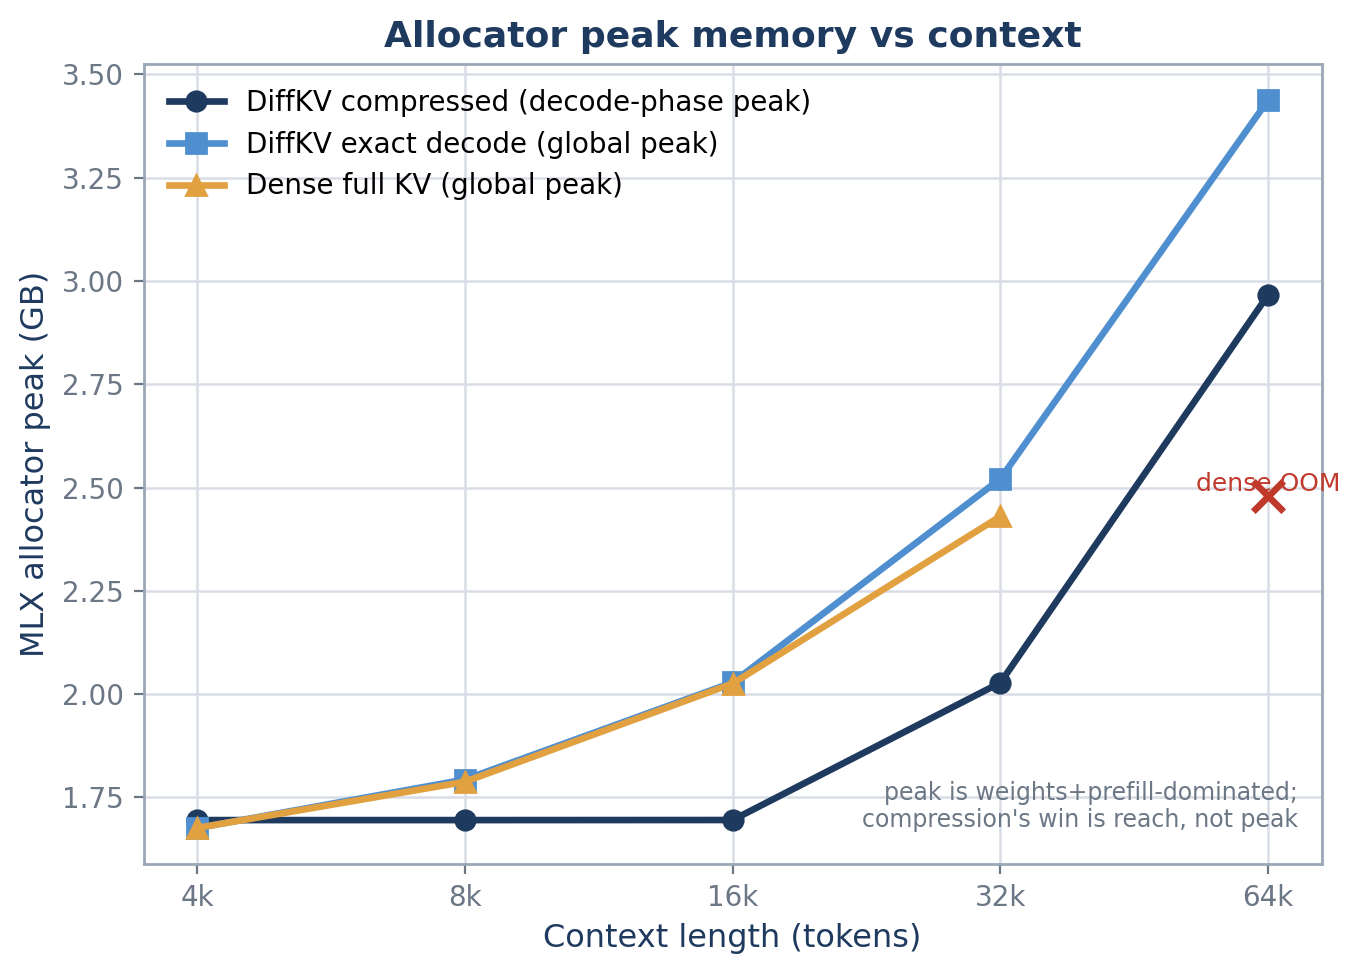
\includegraphics[width=0.92\linewidth]{figures/g2_mx_peak.png}
  \caption{MLX allocator peak vs.\ context. Nearly identical across configurations---peak is
  weights- and prefill-dominated. Compression's win is context reach and steady-state decode
  memory, not the global peak; we report it honestly rather than overstate a peak reduction.}
  \label{fig:g2}
\end{figure}

\begin{figure*}[t]
  \centering
  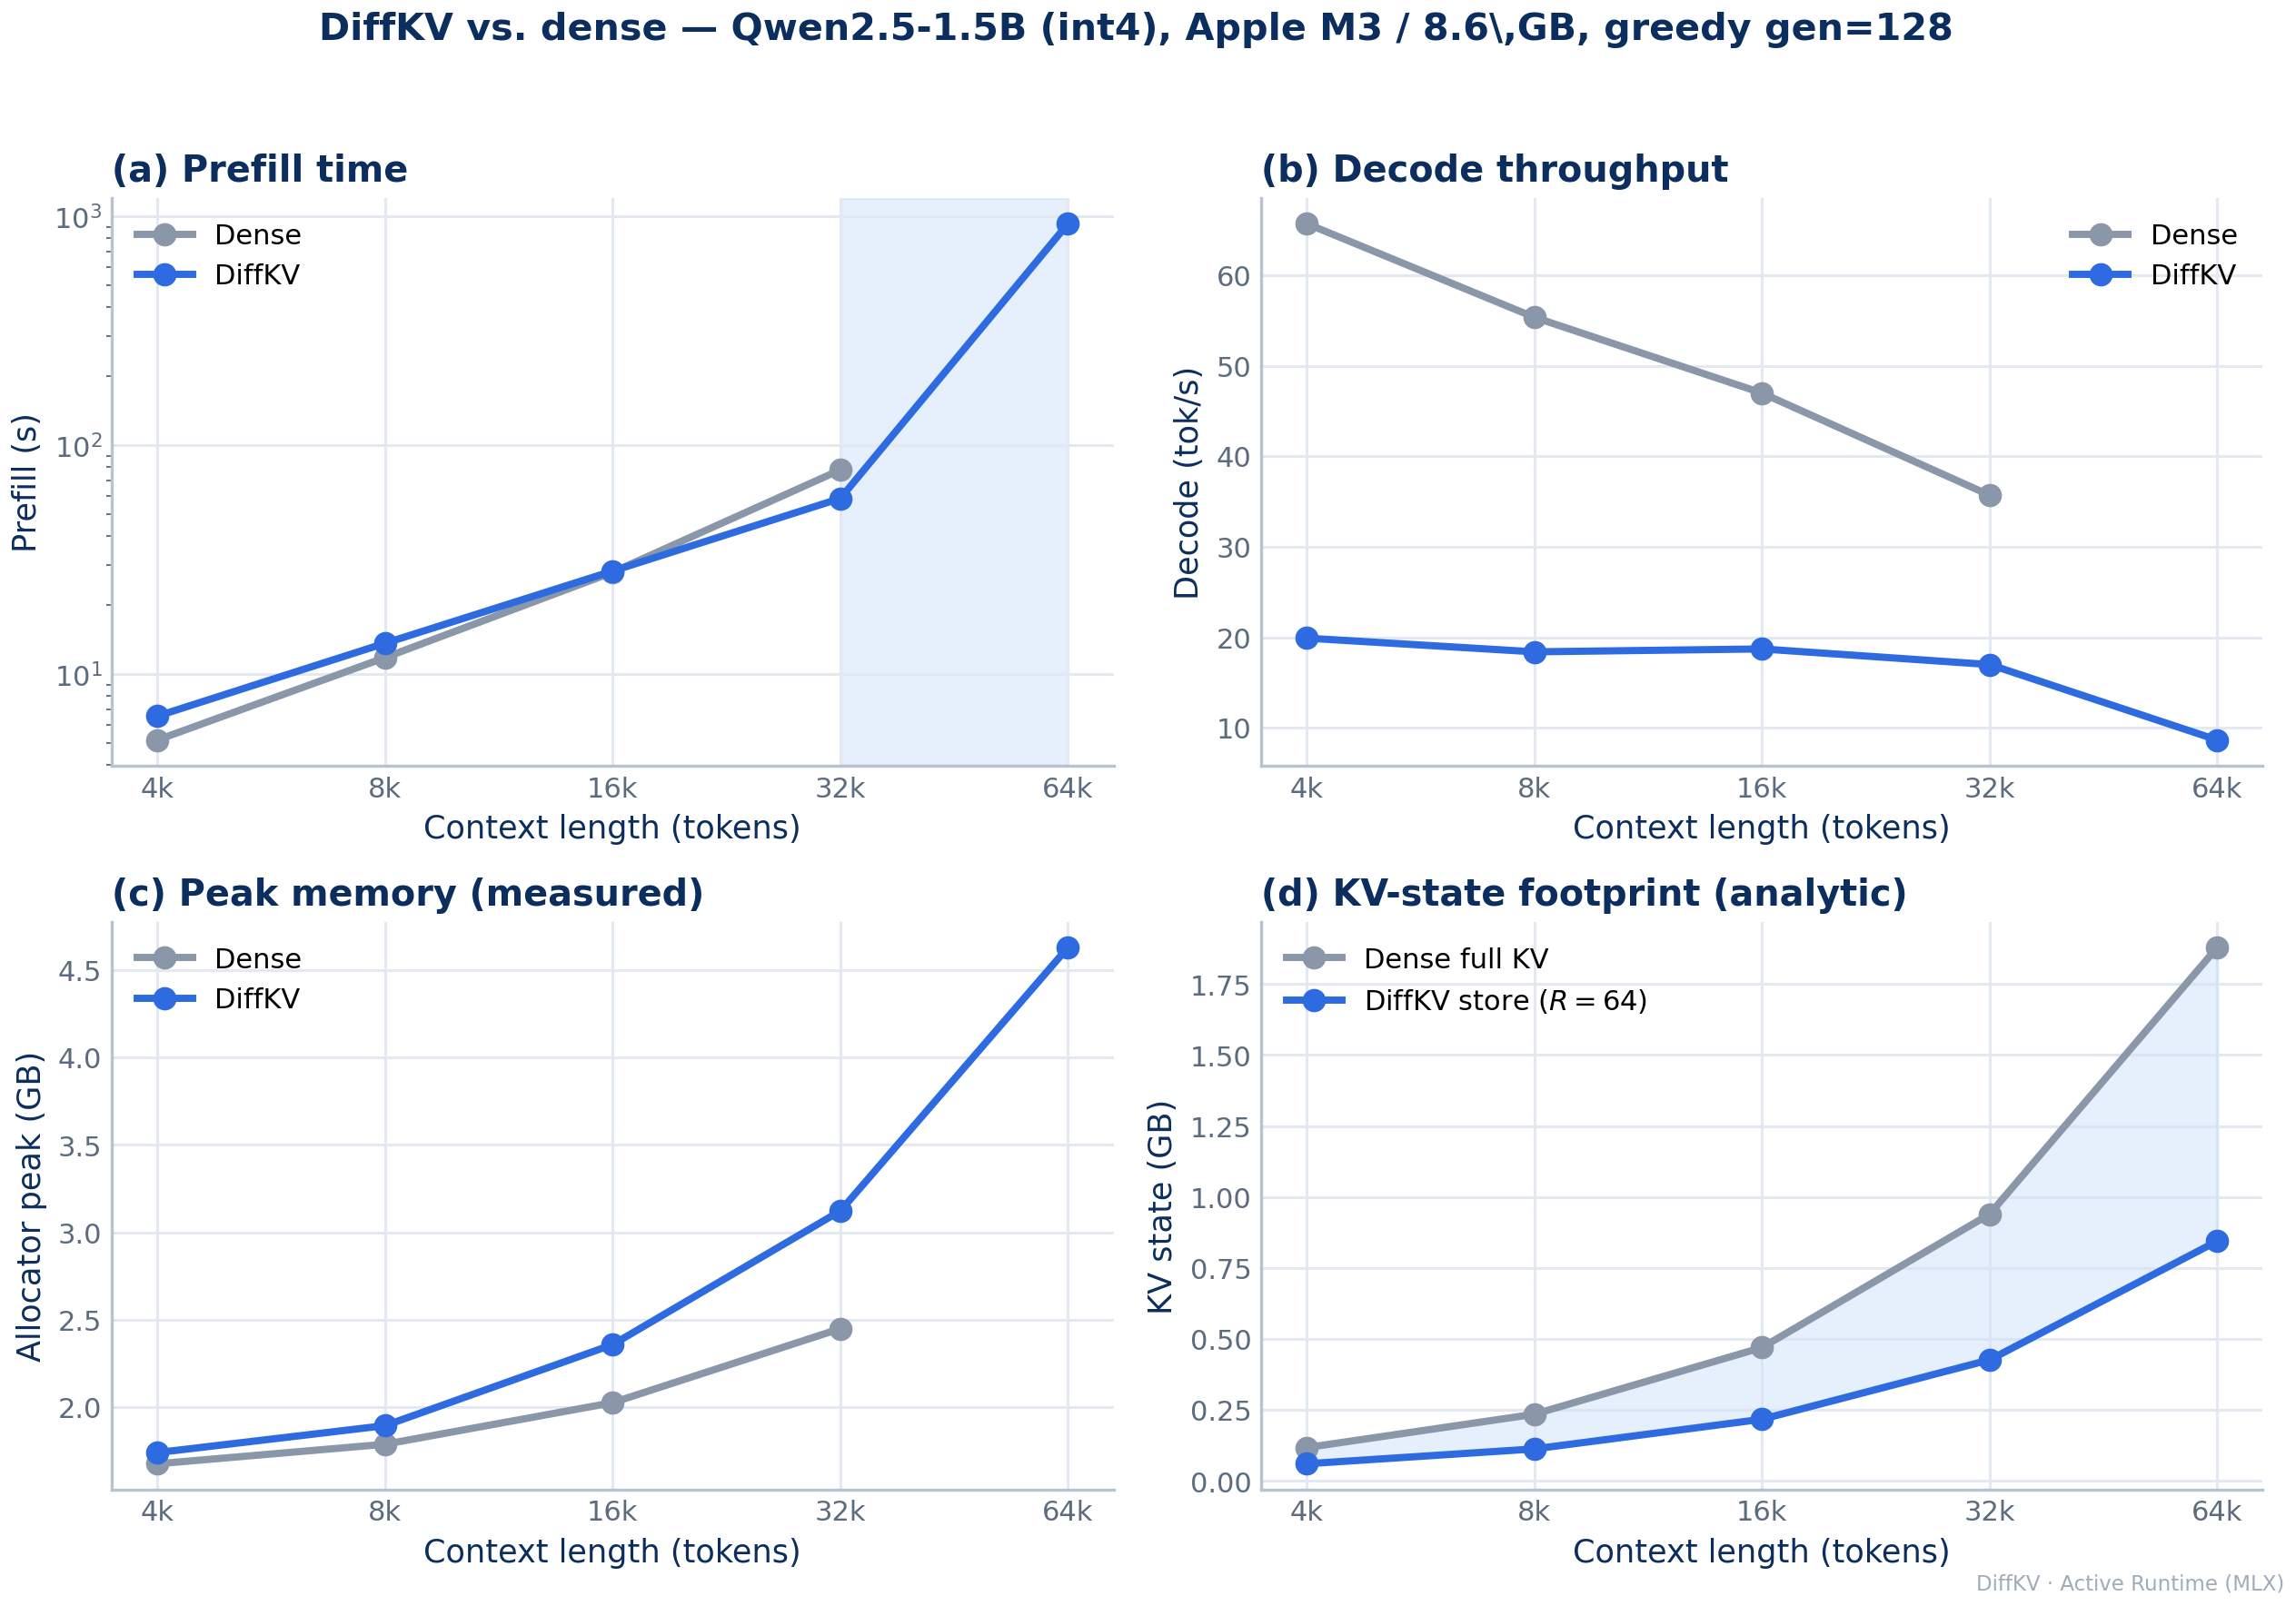
\includegraphics[width=0.96\linewidth]{figures/g5_combined.png}
  \caption{Combined view: (a) KV-state footprint, (b) decode throughput, (c) prefill time, for
  \diffkv{} compressed, the exact ablation, and the dense baseline.}
  \label{fig:g5}
\end{figure*}

\section{Analysis and Discussion}
\label{sec:analysis}

\subsection{What the compression actually buys}
The cleanest statement of \diffkv{}'s benefit is at the level of KV state, not allocator peak.
The compressed store is a \emph{pre-allocated, fixed} pool: its footprint is a constant of the
configuration ($\approx\!0.2$\,GB across $28$ layers) regardless of context, whereas the dense
full-KV cache grows linearly and crosses the store's size early and keeps going
(Fig.~\ref{fig:g1}, Table~\ref{tab:main}). This is the $\rank$-vs-$\Hkv\dhead$ gap of
\S\ref{sec:compression} made concrete: each compressed token carries $O(\rank)$ scalars
instead of $O(\Hkv\dhead)$. Because the store never grows, the runtime addresses contexts the
dense cache cannot fit, which is the qualitative capability the dense baseline lacks at the top
of our range.

\subsection{Why the allocator peak tells a different story}
The MLX allocator peak is nearly identical for the compressed runtime, the exact-decode
ablation, and the dense baseline at matched context, because the peak is set during
\emph{prefill}---a full attention over the growing native cache that all three perform---and is
dominated by weights and transient activations rather than by the retained KV state
(Fig.~\ref{fig:g2}). Compression reduces the \emph{steady-state} decode footprint, not the
prefill peak. We make this explicit rather than reporting only a process-level memory number
that would credit compression with a peak reduction it does not deliver. The practical
implication is that on a memory-constrained device the binding event is whichever is larger of
(a) the prefill peak and (b) the decode-time resident set; \diffkv{} lowers (b) decisively but
leaves (a) to be addressed by prefill-side techniques (chunking, activation release), which the
runtime already applies.

\subsection{The throughput cost}
The compressed decode is several times slower than dense decode and roughly flat across context
(Fig.~\ref{fig:g3}). The flatness is consistent with the compute profile of
\S\ref{sec:decode}: work is linear in the number of \emph{blocks} with a small $\rank$-weighted
constant, so per-token cost rises slowly. The absolute gap is an implementation property, not an
algorithmic necessity: the kernel expresses many small tensor contractions inside one compiled
graph, and on this hardware that does not reach the throughput of MLX's native fused attention
over a contiguous cache. The exact-decode ablation---identical store, but attention computed
over the retained native cache---recovers dense-like throughput, which localizes the gap to the
compressed-kernel dispatch rather than to anything the compression precludes.

\subsection{The fidelity cost}
\label{sec:fidelity}
Under the needle-in-a-haystack probe, the compressed decode does \emph{not} reliably reproduce
the buried passcode once it has left the recency window, whereas the exact-decode ablation on the
same store recovers it at every context (Table~\ref{tab:main}). The exact ablation isolates the
cause: the information needed is present in the recency window when the needle is recent, but
once a needle-bearing block is compressed at rank $16$, the truncated SVD does not preserve the
single-token detail well enough for the query to recover the exact string. This is a property of
rank-$16$ truncation, not of the runtime plumbing---the ablation proves the rest of the path is
correct. We also observe that the compressed output is \emph{non-deterministic} across runs: the
range finder uses an unseeded Gaussian, so different runs produce different (and differently
wrong) reconstructions of a compressed needle. Both are addressable (higher or
adaptive rank, an exact-token residual path, a fixed seed) and are stated as open problems rather
than worked around.

\begin{observation}
\diffkv{} trades \emph{memory and context reach} for \emph{decode throughput and single-token
recall fidelity}. The trade is favorable exactly when the cache is the binding constraint and the
task tolerates approximate long-range recall; it is unfavorable when the device has memory to
spare or the task demands verbatim recall of compressed detail.
\end{observation}

\section{Limitations and Future Work}
\label{sec:limitations}

\paragraph{Decode throughput (primary).}
The fused kernel is expressed as many small ops in a compiled graph and does not yet match native
fused attention (\S\ref{sec:analysis}); the exact-decode ablation localizes the gap to the kernel
dispatch, not the algorithm. A hand-written fused decode---a custom Metal op, or a CUDA/Triton
kernel on NVIDIA hardware---is the natural path to closing it. We have deliberately structured the
throughput figures and the main results table so that a future \textbf{CUDA/Triton fused-decode}
measurement can be added as one more series without restructuring the evaluation; no such number is
reported or estimated here, and the placeholder is labelled as future work. Until then, the
adaptive policy keeps the cost off the short-context path entirely.

\paragraph{Compression ratio and the residual memory ceiling.}
Exact recall is bought with memory: at the default budget a quarter of every block is stored
verbatim, so the per-block reduction is $\approx\!2.85\times$, not the order of magnitude a pure
low-rank scheme suggests (\S\ref{sec:compression}). The residuals also set a scaling ceiling---at a
million tokens the residual K/V alone would dominate the pool---so very long contexts need either a
smaller budget (trading recall, per E6) or a two-stage router that gathers residuals only for
selected blocks (which the runtime already does at decode, but the store still holds them). A
budget that adapts to per-block content, rather than a fixed $\maxres$, is the natural refinement.

\paragraph{Router cost.}
The default residual-key router scores every block's anchor and top residual keys each step, an
$O(nR\dhead)$ cost linear in context. It is cheap relative to the kernel at the scales we test, but
at extreme context a cheap pre-filter feeding the exact rerank would be needed---taking care that
the pre-filter cannot drop the needle's block, the failure mode that motivated the exact router in
the first place.

\paragraph{Prefill cost and peak.}
Prefill remains exact and therefore $O(N)$ in attention, with the per-block SVD and residual
extraction added on top, making it the slowest phase and the dominant wall-time cost at large
context. The global memory peak is also set during prefill (\S\ref{sec:analysis}); \diffkv{} does
not reduce it. Compressed or sparse prefill is a known direction (prototyped in the repository) but
is out of scope here.

\paragraph{Evaluation breadth.}
We report one model (Qwen2.5-1.5B int4), one device (Apple~M3, $8.6$\,GB), and one probe
(needle-in-a-haystack) with greedy decoding. Exact-string recall is a sharp but narrow correctness
signal; broader claims require additional models and sizes, perplexity and downstream-quality
metrics, multi-needle and varied-depth probes, and batched/multi-session throughput. The serving
stack supports batching and multi-session residency; we did not exercise them here.

\paragraph{The grounding module.}
The semantic-retrieval/factual-binding layer is inactive in the benchmarked runtime
(\S\ref{sec:impl}). Whether it improves grounded long-context QA on top of the compressed cache
is an open, separately evaluable question.

\paragraph{Portability.}
The runtime is specialized to MLX and to the Qwen2 attention module it patches. A portable
PyTorch/Triton backend and a C++/GGML reimplementation target the same design in the repository but
are under active development and are not evaluated here.

\section{Conclusion}
\label{sec:conclusion}

\diffkv{} is a KV-cache compression runtime that separates a block's smooth, shared structure---captured
by an anchor and a rank-\rank{} joint $K\!\mid\!V$ delta---from its distinctive outlier tokens, kept
as exact residuals selected by measured reconstruction error. A fused, routed decode kernel scores
queries in the low-rank subspace without ever decompressing the cache, attends the residuals and a
recency window exactly, and merges the two in log-space; a training-free block-sparse prefill makes
long-context prefill sub-quadratic; and a fixed block pool bounds the memory. Implemented entirely
in MLX and measured on Qwen2.5-1.5B (int4) on an $8.6$\,GB Apple~M3, \diffkv{} holds a bounded KV
state $\ratioDefault\times$--$\ratioPreset\times$ smaller per block than a dense cache, recovers a
buried passcode exactly from $4$k to $\reachK$k, reaches $\reachK$k where the dense full-KV cache
runs out of memory, and overtakes dense on long-context prefill---at a measured cost in decode
throughput, in the regime where a dense cache still fits, that we report in full and localize to
reconstruction-and-merge overhead. The residual budget is an explicit dial between memory, accuracy, and speed. The most
promising next steps are a fused (and GPU-native) decode kernel to narrow the throughput gap, and a
broader evaluation across models, hardware, and standard long-context suites. We have been careful
to claim only what the measurements support: \diffkv{} is a memory-and-prefill instrument for
long context on commodity unified-memory hardware, not a universally faster one.


% ── references ──
\bibliographystyle{plain}
\bibliography{bibliography/references}

% ── appendices ──
\appendix
\section{Reproducibility}
\label{app:repro}

All results were produced on a single machine, one engine per isolated subprocess, with every
number measured (failed cells are reported as failures, never filled with estimates).

\paragraph{Hardware.}
Apple~M3, $8.59$\,GB unified memory (host \texttt{Oms-MacBook-Pro-2.local}), macOS (Darwin
25.x). The device is shared with the OS and other applications, so absolute memory thresholds
shift with machine load; the scaling slopes and engine ordering are the stable results.

\paragraph{Software.}
Python (\texttt{diffkv\_venv}), MLX $0.31.2$, \texttt{mlx\_lm}, NumPy, PyTorch (used only for
tensor plumbing in the wrapper, not for compute), \texttt{psutil}. Model:
\texttt{mlx-community/Qwen2.5-1.5B-Instruct-4bit} (group size $64$, $4$-bit), $28$ layers,
$12$ query heads, $2$ KV heads, head dim $128$, vocab $151{,}936$, trained context $32{,}768$,
RoPE $\theta=10^6$.

\paragraph{Configuration.}
\texttt{rank=16}, \texttt{block\_size=256}, \texttt{recency\_window=512} (dense buffer $768$),
\texttt{max\_blocks=256}, preset ``mid''. Decode mode is selected by
\texttt{DIFFKV\_COMPRESSED\_DECODE} ($1$ = compressed, primary; $0$ = exact, ablation).

\paragraph{Protocol.}
A needle-in-a-haystack chat prompt is built once per context length from the Qwen2.5 tokenizer
and fed verbatim (raw mode, no double chat-templating) to every configuration. The needle is a
planted passcode (\texttt{OMEGA-7741-DELTA}); ``needle recovered'' means the generation
reproduced it---a free correctness signal. Engines are warmed once (a $1$-token forward to
compile kernels) before timing. Prefill is timed with \texttt{perf\_counter} around the chunked
forward after \texttt{mx.eval}; decode is fixed-length greedy ($128$ tokens, EOS ignored) so
throughput is directly comparable. Memory is read from MLX's allocator
(\texttt{get\_peak\_memory}/\texttt{get\_active\_memory}); the decode-phase peak resets the peak
counter at the prefill$\to$decode boundary to isolate steady-state decode memory. Analytic
KV-state bytes are computed from the live store occupancy.

\paragraph{Commands.}
\begin{quote}\small\ttfamily
\# instrumented active sweep (compressed + exact ablation)\\
diffkv\_venv/bin/python3 paper/scripts/measure\_active.py \textbackslash\\
\ \ --ctx 4096 8192 16384 32768 65536 --modes compressed exact \textbackslash\\
\ \ --gen 128 --out paper/generated/active\_modes\_sweep.json\\[4pt]
\# dense full-KV baseline (same prompts, same memory metric)\\
diffkv\_venv/bin/python3 benchmarks/run\_bench.py --engines dense \textbackslash\\
\ \ --contexts 4096 8192 16384 32768 --gen 128 --ram-cap-gb 7.5\\[4pt]
\# figures + tables from the measured JSON\\
diffkv\_venv/bin/python3 paper/scripts/make\_diagrams.py\\
diffkv\_venv/bin/python3 paper/scripts/make\_graphs.py\\
diffkv\_venv/bin/python3 paper/scripts/make\_tables.py
\end{quote}

\paragraph{Artifacts.}
Measured JSON: \texttt{paper/generated/active\_modes\_sweep.json} (active, both modes) and
\texttt{benchmarks/results/PAPER\_dense\_sweep.json} (dense). Figures are regenerated from these
by the scripts above; tables are emitted to \texttt{paper/tables/}. The provenance and the
decode-path conflict that motivated this measurement design are documented in
\texttt{paper/notes/}.

\section{Full Measured Results}
\label{app:tables}

Table~\ref{tab:detail} lists every measured cell from the instrumented sweep
(\texttt{paper/scripts/measure\_active.py}) and the dense baseline
(\texttt{benchmarks/run\_bench.py}). \emph{Decode-phase peak} resets the MLX peak counter at
the prefill$\to$decode boundary to isolate steady-state decode memory; \emph{Store} is the
analytic occupied KV-state footprint of the compressed pool plus recency window; \emph{Full KV}
is the analytic dense-cache size for the same sequence length (all $28$ layers, fp16). Empty
cells are measurements that do not apply to that configuration; failed cells (e.g.\ a dense
out-of-memory at $64$k) are stated in the text, never given an invented value.

\begin{table}[h]
\centering
\caption{Per-run detail: compressed decode (primary), exact decode (ablation), dense baseline.}
\label{tab:detail}
\small
\begin{tabular}{llrrrrl}
\toprule
Engine & Ctx & Prompt tok & Prefill (s) & Decode (tok/s) & MLX peak (GB) & Needle \\
\midrule
active & 4k & 4096 & 6.6 & 19.9 & 1.74 & \cmark \\
active & 8k & 8192 & 13.6 & 18.4 & 1.89 & \cmark \\
active & 16k & 16490 & 28.2 & 18.7 & 2.36 & \cmark \\
active & 32k & 32865 & 58.5 & 17.0 & 3.12 & \cmark \\
active & 64k & 65615 & 928.0 & 8.6 & 4.63 & \cmark \\
\midrule
dense & 4k & 4096 & 5.1 & 65.7 & 1.68 & \cmark \\
dense & 8k & 8192 & 11.8 & 55.3 & 1.79 & \cmark \\
dense & 16k & 16490 & 27.8 & 47.0 & 2.03 & \cmark \\
dense & 32k & 32865 & 77.9 & 35.7 & 2.45 & \cmark \\
\bottomrule
\end{tabular}

\end{table}

\section{Notation}
\label{app:notation}

\begin{center}
\begin{tabular}{ll}
\toprule
Symbol & Meaning \\
\midrule
$L$ & transformer layers ($28$) \\
$H$ & query heads ($12$) \\
$\Hkv$ & key/value heads ($2$) \\
$G=H/\Hkv$ & GQA group size ($6$) \\
$\dhead$ & head dimension ($128$) \\
$N$ & sequence length (tokens) \\
$\bs$ & block size ($256$) \\
$S=\bs-1$ & compressible tokens per block ($255$) \\
$\rank$ & SVD target rank ($16$; adaptive in $[4,\rank]$) \\
$\dwin$ & dense recency window ($512$; buffer $\dwin{+}\bs=768$) \\
$M$ & compressed-pool capacity ($256$ blocks) \\
$\anchork,\anchorv$ & anchor key / value (token $0$ of a block) \\
$U$ & per-token coefficients $\R^{S\times\rank}$ (shared K/V) \\
$V_K,V_V$ & key / value bases $\R^{\Hkv\times\rank\times\dhead}$ \\
$s$ & SVD normalization scale (fp32) \\
$q,\sigma$ & query, attention scale \\
$\ell^{\text{sp}},\ell^{\text{dn}}$ & log-sum-exp of compressed / dense branch \\
\bottomrule
\end{tabular}
\end{center}


\end{document}
